\chapter{Jet Algorithms for the L1 Trigger Upgrade}
\label{chap:l1jets}

In the hadron rich environment of the \ac{LHC}, \added{jets are very important}. 
Whether for \ac{SM} analyses, Higgs searches, \ac{SUSY} searches or exotic analyses,
jet reconstruction is vital for both online event selection and offline analysis, for a wide range of kinematic requirements.
Efficient and reliable triggering on jets is therefore of key importance
and the first stage of event selection, the \ac{L1} trigger, must have an effective jet algorithm. 
This is of particular significance as we look towards the \ac{LHC} upgrade, when running conditions become increasingly challenging. 
Up to double the instantaneous luminosity and centre-of-mass energy lead to an increase in \ac{PU} up to $\sim 70$ and far higher detector occupancies.
Jet algorithms must maintain a similar performance in this next phase of \ac{LHC} running as exhibited in the previous period of data collection.
A new \ac{L1} jet algorithm is proposed, which exploits the full granularity of the calorimeter and uses event-by-event \ac{PU} subtraction. 

\section{The LHC Upgrade\label{sec:LHCupgrade}}


\added{
There are various phases of planned \ac{LHC} upgrades, as discussed in Chapter~\ref{chap:detector}. 
The algorithm described in this chapter is for implementation in Run 2, from 2016.
The new trigger architecture is being installed during LS1, and the system will be commissioned during 2015 (the first year of Run 2), ready to be brought online in 2016 when it will replace the current system. 
The two trigger systems (current and upgrade) will run in parallel during 2015, to make sure that CMS is never without a functional L1 trigger. 
}

\subsection{Motivations for a new L1 jet algorithm}

If\added{, during Run 2,} the machine operates at 50~\ns, the instantaneous luminosity will double compared to that of Run 1, with PU expected to more than double from around 20 inelastic collisions per bunch crossing to, perhaps, in excess of 70.
%As a result, the number of interactions per second will also increase; and detector occupancies and trigger rates will soar.
Not only will the number of interactions per second increase due to the higher instantaneous luminosity, but the increased centre of mass energy means the energy of these interactions will also increase. 
Consequently, for a particular trigger (say, for example a single jet trigger), many, many more events will pass a particular energy threshold as compared to Run 1. 
As a result, the trigger rate will soar.

For a single jet trigger, where the jet (reconstructed offline) is required to be above 128~\GeV, 95\% of jets which have been matched to this offline jet and reconstructed using the existing \ac{L1} jet algorithm are above 150~\GeV --- where the higher \ac{L1} threshold is due to poorer \ac{L1} reconstruction than offline reconstruction. 
In a typical \added{Run 1} run during 2012 (PU=15, $\mathcal{L}=0.4 \times 10^{34}$~cm$^{-2}$s$^{-1}$), a \ac{L1} jet threshold of 150~\GeV corresponds to a rate of 1.1~\kHz.
In the high \ac{PU} test runs during 2012, 
%that had a few bunches filled which could then be scaled up to high luminosity and \ac{PU}, 
this trigger rate rose to 3.6~\kHz (PU=45, $\mathcal{L}=1.1 \times 10^{34}$cm$^{-2}$s$^{-1}$ equivalent); and simulation shows that in similar conditions but at 14~\TeV, a trigger rate of 14~\kHz is expected.
The total rate of all of the \ac{L1} triggers is capped at 100~\kHz by design, 
and a balanced trigger menu is desirable to satisfy all of the physics demands of \ac{CMS}.
Therefore, individual trigger rates must be kept reasonably low to ensure the total \ac{L1} trigger rate is acceptable.  
The only way to maintain low trigger rates in the more challenging run conditions is to increase energy thresholds.
Figure~\ref{tab:L1TrigMenuCurrentSystem} shows an illustrative \ac{L1} trigger menu for the upgraded \ac{LHC} \added{during Run 2}, for two luminosity scenarios which have bunch spacings of 50~\ns (centre column) and 50~\ns (right column). 
Thresholds have had to be significantly raised to maintain a total rate below 100~\kHz; for example, the single jet threshold is increased \added{from 128~\GeV in Run 1} to 170~\GeV and 205~\GeV for 50 and 25~\ns bunch crossings respectively.


\begin{figure}[htbp]
  \begin{center}
  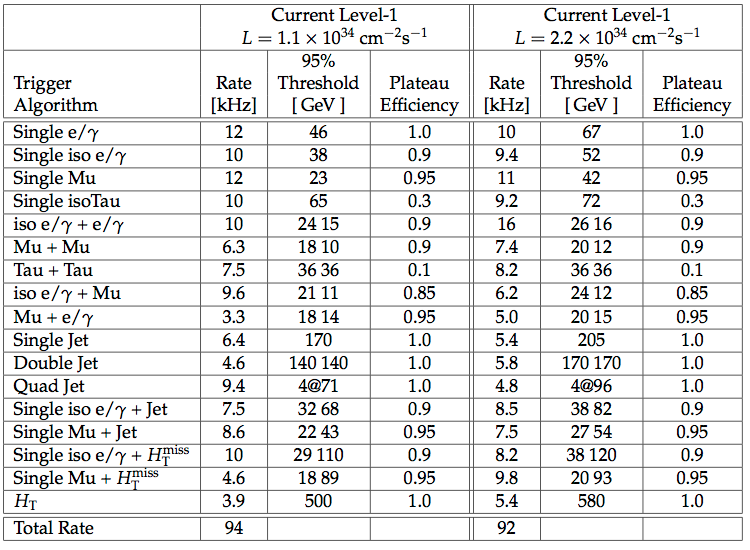
\includegraphics[width=0.95\textwidth]{Figures/l1jets/triggerThresholdCurrentL1Table.png}
  \caption{A possible \added{Run 2} \ac{L1} trigger menu, using the current \ac{L1} system and algorithms, \added{where $\sqrt{s} =$} 14~\TeV~\cite{Tapper:1556311}. 
  \added{The numbers here are for illustration purposes only - they are not a proposed trigger menu. }
  In the left hand column, all of the different triggers contributing to the menu are shown. 
  In the centre (right-hand) columns, the projected L1 trigger rate, 95\% threshold and plateau efficiency are shown for \added{possible Run 2} running conditions with bunch spacing of 50~\ns, $\mathcal{L}=1.1 \times 10^{34}$~cm$^{-2}$s$^{-1}$, PU=50 (25~ns, $\mathcal{L}=2.2 \times 10^{34}$~cm$^{-2}$s$^{-1}$, PU=50).
}
  \label{tab:L1TrigMenuCurrentSystem}
  \end{center}
\end{figure}


For the physics requirements of \ac{CMS} the necessary increase in \ac{L1} thresholds, and corresponding increase in offline (analysis) thresholds, is an unacceptable compromise as lower energy final states are crucial to many analyses and keeping as much physics, at as low thresholds as possible, is desirable.
To cope with the challenges of the \ac{LHC} upgrades, and to enable new algorithms (with better performance) to be developed so the physics performance of Run 1 can be maintained, or bettered, the \ac{CMS} \ac{L1} trigger is undergoing upgrades. 



\section{CMS Trigger Upgrade}
Upgrades to the electronics of the calorimeter trigger, muon trigger and global trigger are under way in order 
to meet the triggering demands of \ac{CMS}.
These upgrades involve installing additional interconnections between the systems, reducing the current huge diversity of electronics cards to a small number of multi-purpose and adaptable cards, using high bandwidth optical links and modern, high powered \ac{FPGA} processing chips. 
These upgrades not only allow more information from the detector subsystems to be used as inputs to improved (more sophisticated) algorithms, due to increased logic resources and fast links, 
but crucially also allow far more flexibility in the \ac{L1} trigger system. 
In Run 1, the ability to adapt the trigger algorithms and menu to evolving \ac{LHC} run conditions proved vital in reducing trigger rates and improving efficiencies. 
Increasing the flexibility by making more of the system adaptable, and more of the cards standardised, will only improve the trigger and enhance its longevity. 
Having the ability to easily update software and firmware, as well as trigger architecture, in response to unforeseen circumstances --- not just in the planned \ac{LHC} upgrades to 2016 but far beyond --- will put \ac{CMS} in an excellent position for data collection.

The new \ac{L1} trigger is being installed during \ac{LS1}, and will be commissioned and run concurrently with the existing trigger during Run 2. 
%Once it's performance has been tested and verified, 
The upgraded system will be available for physics in 2016. %, and after LS2 at which point the existing system will no longer be operable.
Here, I discuss in detail the calorimeter trigger upgrade, as this is what the proposed jet algorithm, detailed in this chapter, relies upon.
More information on the muon trigger and global trigger upgrade can be found in Ref.~\cite{Tapper:1556311}.



\subsection{Calorimeter trigger upgrade}
The calorimeter trigger uses information from the \ac{ECAL} and \ac{HCAL} to look for electrons/photons and jets, as described in the previous chapter.
It currently is based upon a traditional trigger design; where the detector is spatially segmented into different processing nodes, each of which deals with the data from each geographical region, and does so at every bunch crossing.
The desire for far more flexibility in triggering motivates a new approach to the upgrade trigger architecture, known as time-multiplexing.
Instead of splitting the detector into geographical regions and sending the data to different processors at every bunch crossing, 
a \ac{TMT}~\cite{TMT_dem} places all of the data from the detector in a single processor across several bunch crossings.
No data are thrown away at any stage of the process, and all of the data, at its full granularity, is available in the same card making many more algorithms possible.


\subsubsection{Traditional trigger architecture}
A conventional trigger architecture is shown in Figure~\ref{fig:tradTrig}.
The calorimeter is split into geographical regions in $\eta-\phi$, 
and at every bunch crossing data from the individual regions are sent to different processors.
Boundaries between these regions must be duplicated in each implicated processor, to ensure that any objects found along the boundary are sufficiently dealt with.
To achieve a compact implementation, at each stage of the trigger process the volume of data is reduced and the minimal information with which to make a decision is passed onto the \ac{GT}. 
Therefore, a lot of the information from an event is discarded before a decision at the \ac{GT} is made.
In addition, the current calorimeter trigger does not use the full granularity of information available, and the combined \ac{ASIC} and \ac{FPGA} hardware, although permitting some flexibility in algorithms and parameters, is restricted by a fixed data flow. 
Not all algorithms can therefore be implemented, and the coarse inputs limit the possible performance.

\begin{figure}[h!]
%\vspace{-1.cm}
\begin{center}
  \includegraphics[scale=0.78]{Figures/l1jets/TraditionalTrigger.png}
\caption{Conventional trigger architecture, showing data processing in regions~\cite{RoseTrig}.\added{ Here, and in Figure~\ref{fig:TMTrig}, `TPG' stands for trigger primitive generators.}}
\label{fig:tradTrig}
\end{center}
\end{figure}

Energy clusters are built into physics objects with which the \ac{GT} can make a decision over two processing layers. 
Trigger towers, consisting of groups of $5 \times 5$ crystals in the \ac{ECAL}, and the corresponding blocks of the \ac{HCAL}, are themselves grouped into $4 \times 4$ arrays or ``regions''. 
These regions are used as inputs to the various object algorithms.
In the first layer, the `Regional stages' in Figure~\ref{fig:tradTrig}, the regions, or clusters of transverse energy are assigned a type; electron/photon-like, if the energy is predominantly in the \ac{ECAL}, otherwise hadron-like.
In the second processing layer, the `Global Stages', the cluster type is identified as an electron/photon or tau (for high energy or isolated deposits respectively), and non-isolated clusters are grouped together to form jets.
The jet finding algorithm looks for energy deposits in windows of $3 \times 3$ regions, with the requirement that the central region has a larger transverse energy deposit. 
The top four candidates are passed onto the global trigger, with the rest discarded.
Also in this layer of processing, the value and direction of the total missing transverse momentum are calculated from the sum of energy deposits across the calorimeter, 
and jet candidates above threshold are summed to give the total hadronic energy content, known as $H_{\mathrm{T}}$.    




\subsubsection{Time multiplexed trigger}
A time-multiplexed trigger architecture is shown in Figure~\ref{fig:TMTrig}. 
In a similar way as the \ac{HLT}, it will consist of parallel nodes, each of which process individual events concurrently~\cite{TMT_dem}.
All of the data from an event --- from the whole $\eta - \phi$ range of the calorimeter and at full granularity --- are sent to an individual processor. 
The first processor receives the data from the first bunch crossing over $N$ clock cycles (where the length of a clock cycle is equal to the time between bunch crossings, 25 or 50~\ns).
The data from the second bunch crossing are sent to the second processor, again over $N$ clock cycles, and so on; where there are more than $N$ processors in total, as each processor needs time to process each event.
After the first processor has processed all of the data from the first bunch crossing and passed it on to the next stage of the trigger, the `Demux' in Figure~\ref{fig:TMTrig} (some $N+X$ clock cycles after the first bunch crossing where $X$ is the time taken to process and send on the data), it can then receive data from another bunch crossing.
Developments in large \ac{FPGA} chips and increased rate and volume of data transmission in optical fibres make this kind of architecture possible for the upgraded \ac{CMS} \ac{L1} calorimeter trigger, whereas it was not when the current trigger was designed and built. 
The system latency, $N+X$, is now small enough, due to the increased processing power and bandwidths, that it is viable in hardware for the huge amounts of data and short time-scale that the trigger demands~\cite{TMT_dem}. 

\begin{figure}[h]
%\vspace{-1.cm}
\begin{center}
  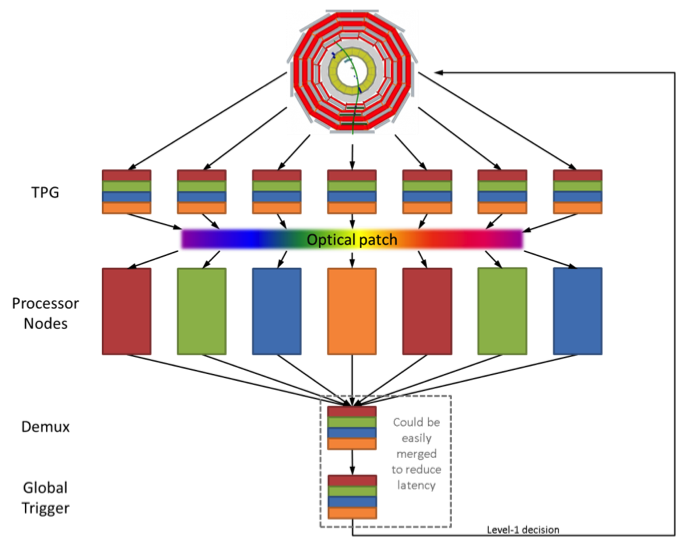
\includegraphics[scale=0.8]{Figures/l1jets/TMTrigger.png}

\caption{Time-multiplexed trigger architecture, showing data pipe-lining to different processing nodes~\cite{RoseTrig}. }
\label{fig:TMTrig}
\end{center}
\end{figure}


With all of the data, at full granularity, in one single processor, many more algorithms for object reconstruction are possible. 
Tower level calorimeter inputs (rather than region level inputs) will be available, increasing the granularity by a factor of 4$^{2}$, with similarly improved spatial resolutions.
There is also scope for an array of additional variables, using information from the whole calorimeter. For example, the average energy deposit for each row in $|\eta|$ or ring of $\phi$ can be calculated, and used to give an estimate of \ac{PU} on an event-by-event basis.
In the remainder of this chapter, a jet algorithm is proposed for the upgraded \ac{L1} calorimeter trigger.
More detail on the CMS \ac{L1} calorimeter trigger upgrade can be found in Ref.~\cite{1748-0221-9-01-C01006}.


%%%%%%%%%%%%%%%%%%%%%%%%%%%%%%%%%%%%%%%%%%%%%%%%%%%%%%%%%%%%%%%%%%%%%%%%%%%%%%%%%%%%%%%%%%%%%%%
%        _ ______ _______            _      _____  ____  _____  _____ _______ _    _ __  __ 
%       | |  ____|__   __|     /\   | |    / ____|/ __ \|  __ \|_   _|__   __| |  | |  \/  |
%       | | |__     | |       /  \  | |   | |  __| |  | | |__) | | |    | |  | |__| | \  / |
%   _   | |  __|    | |      / /\ \ | |   | | |_ | |  | |  _  /  | |    | |  |  __  | |\/| |
%  | |__| | |____   | |     / ____ \| |___| |__| | |__| | | \ \ _| |_   | |  | |  | | |  | |
%   \____/|______|  |_|    /_/    \_\______\_____|\____/|_|  \_\_____|  |_|  |_|  |_|_|  |_|
%        
%%%%%%%%%%%%%%%%%%%%%%%%%%%%%%%%%%%%%%%%%%%%%%%%%%%%%%%%%%%%%%%%%%%%%%%%%%%%%%%%%%%%%%%%%%%%%%%

\section{Algorithm for Jet Reconstruction at L1}
\label{Sec:Algo}
A jet algorithm to reconstruct, filter and calibrate \ac{L1} jets is proposed, for the upgraded \ac{CMS} calorimeter trigger.
It is assumed that all of the \ac{L1} calorimetric information for a single event streams through a single processor; that is, all of the information from a single bunch crossing can be processed in one single chip.
This is compatible with the \ac{TMT} architecture which will be available after \replaced{\ac{LS1} at \ac{CMS}, ready to be brought online fully in 2016}{LS2 at CMS}. 

Using tower level information, the algorithm creates a tunable sized jet at each site on the calorimeter, filters out zero-energy jets and repeats, to get the `best' 13 jet candidates per event. 
The \replaced{median}{average} jet energy density for each event is calculated, and subtracted from the energy deposited across the calorimeter in order to perform \ac{PU} subtraction on an event-by-event basis. 
The 13 jet candidates are then calibrated to offline energy. 
This algorithm is compared to the current \ac{L1} jet algorithm: a much improved spatial resolution is seen, as well as enhanced, and crucially, more \ac{PU} independent, energy resolution. 
The resulting trigger turn-on curves for various jet energy thresholds, and trigger rates for single and multijet triggers are improved compared to the current algorithm, as well as rates for the global variable \HT trigger.
This jet algorithm was the proposed jet algorithm in the \ac{CMS} \ac{L1} Trigger Upgrade Technical Design Review, Ref.~\cite{Tapper:1556311}. 
\added{
With help from A. Rose for the initial algorithm idea, the author was responsible for all of the work that follows on this jet algorithm: designing and implementing the algorithm, refining and testing it, calibrating the jets, and characterizing performance.
}


\subsection{Jet reconstruction}

The proposed jet algorithm uses the full granularity of the calorimeters available at \ac{L1}; that is, $5 \times 5$ \ac{ECAL} crystals grouped together into towers, with the corresponding block of \ac{HCAL}. 
In the centre of \ac{CMS}, each tower measures $0.087\times0.087$ in the $\eta-\phi$ plane, with the $\eta$ dimension increasing as $\eta$ increases; see Figure~\ref{fig:towerGeo}. 
In total there are 72 towers in the $\phi$ direction, and for $|\eta|\leq3.0$ (the barrel region), 56 towers in the $\eta$ direction.
The sum of energy deposits in both the \ac{ECAL} and \ac{HCAL} at each tower is used as input to the algorithm. 

\begin{figure}[ht]
%\vspace{-1.cm}
\begin{center}
  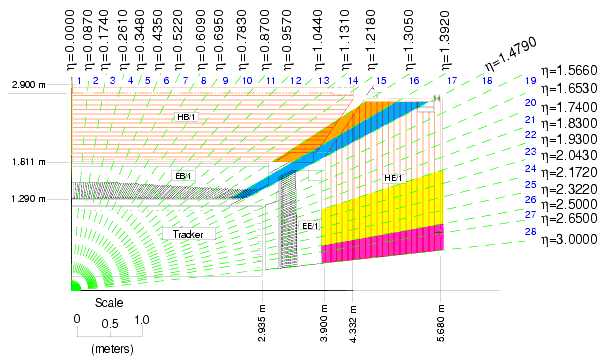
\includegraphics[scale=0.67]{Figures/l1jets/towerGeometry}

\caption{Layout of trigger towers in the $r-z$ projection, for $0<\eta<3.0$. Both \ac{ECAL} and \ac{HCAL} towers are shown.}
\label{fig:towerGeo}
\end{center}
\end{figure}

A group of $n \times n$ towers is combined to form a jet candidate, where the energy of that jet candidate is the sum of the $n \times n$ towers it consists of. 
The jet size, $n$, is completely flexible, as well as the jet shape. 
Jet sizes of $8\times8$ to $12\times12$ were studied, and both circular and square jets. 
This compares with the current \ac{L1} jet algorithm, which consists of equivalent $12\times12$ square jets 
- where the towers are incorporated into regions, each measuring $4\times4$ towers; see Figure~\ref{fig:jetcartoon} for a comparison of the current and proposed upgrade jet geometry.
For circular jets the size $n$ represents the length of the diameter, 
for square jets it represents the length of the side. 

\begin{figure}[ht]
%\vspace{-1.cm}
\begin{center}
  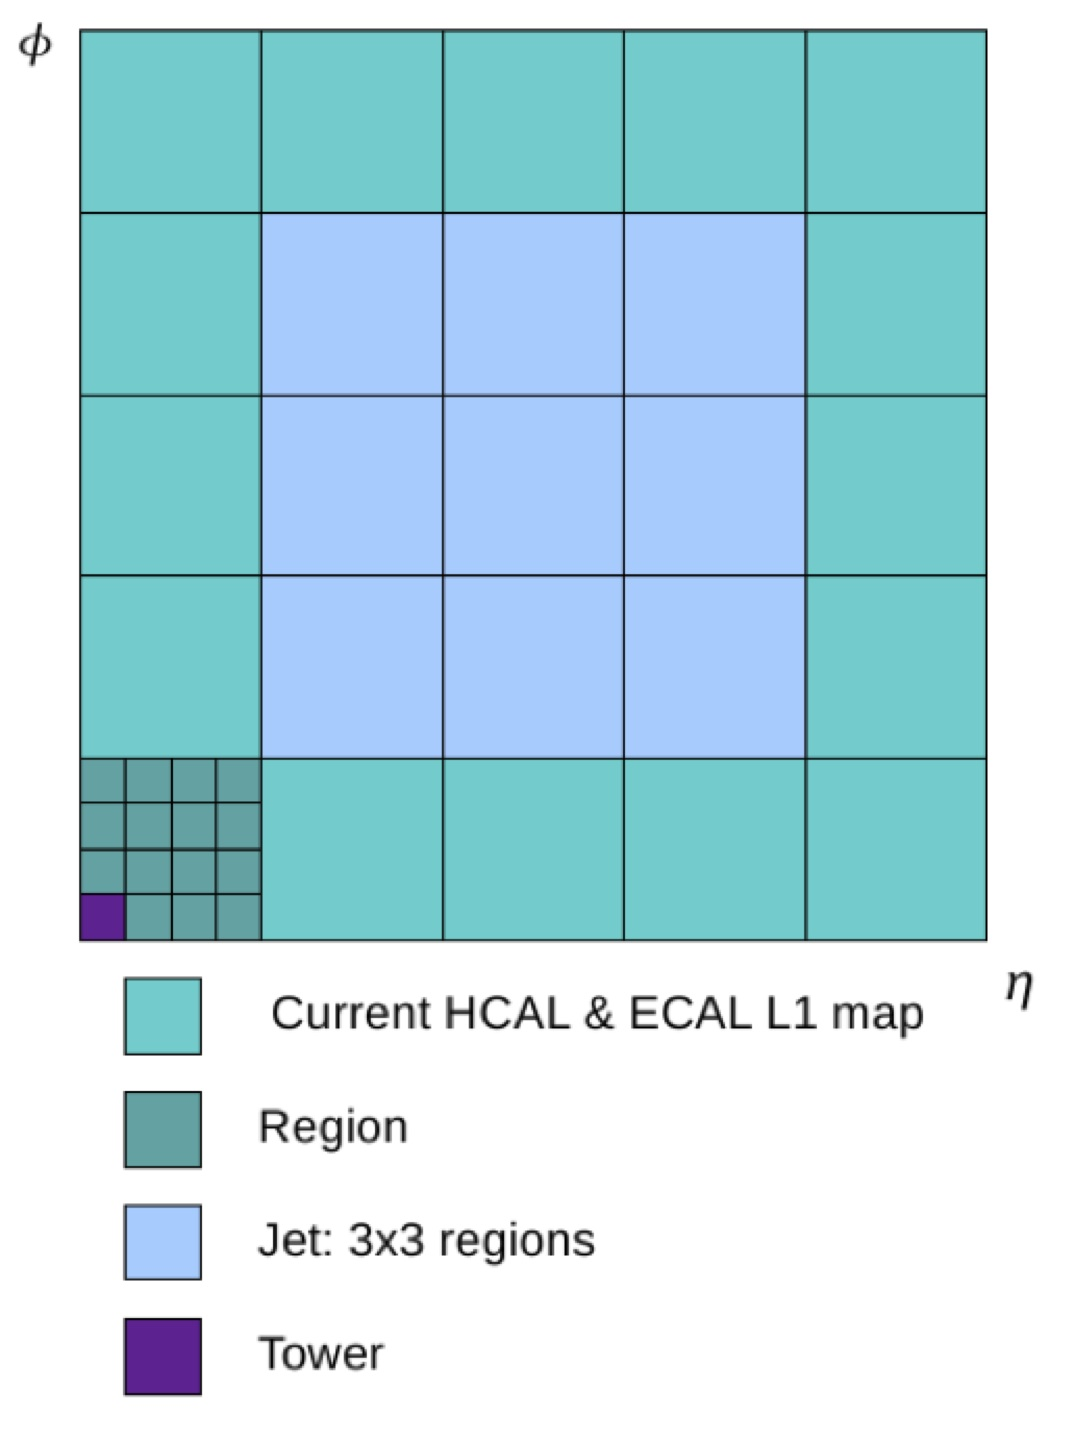
\includegraphics[scale=0.34]{Figures/l1jets/CurrentL1Jet.jpg}
  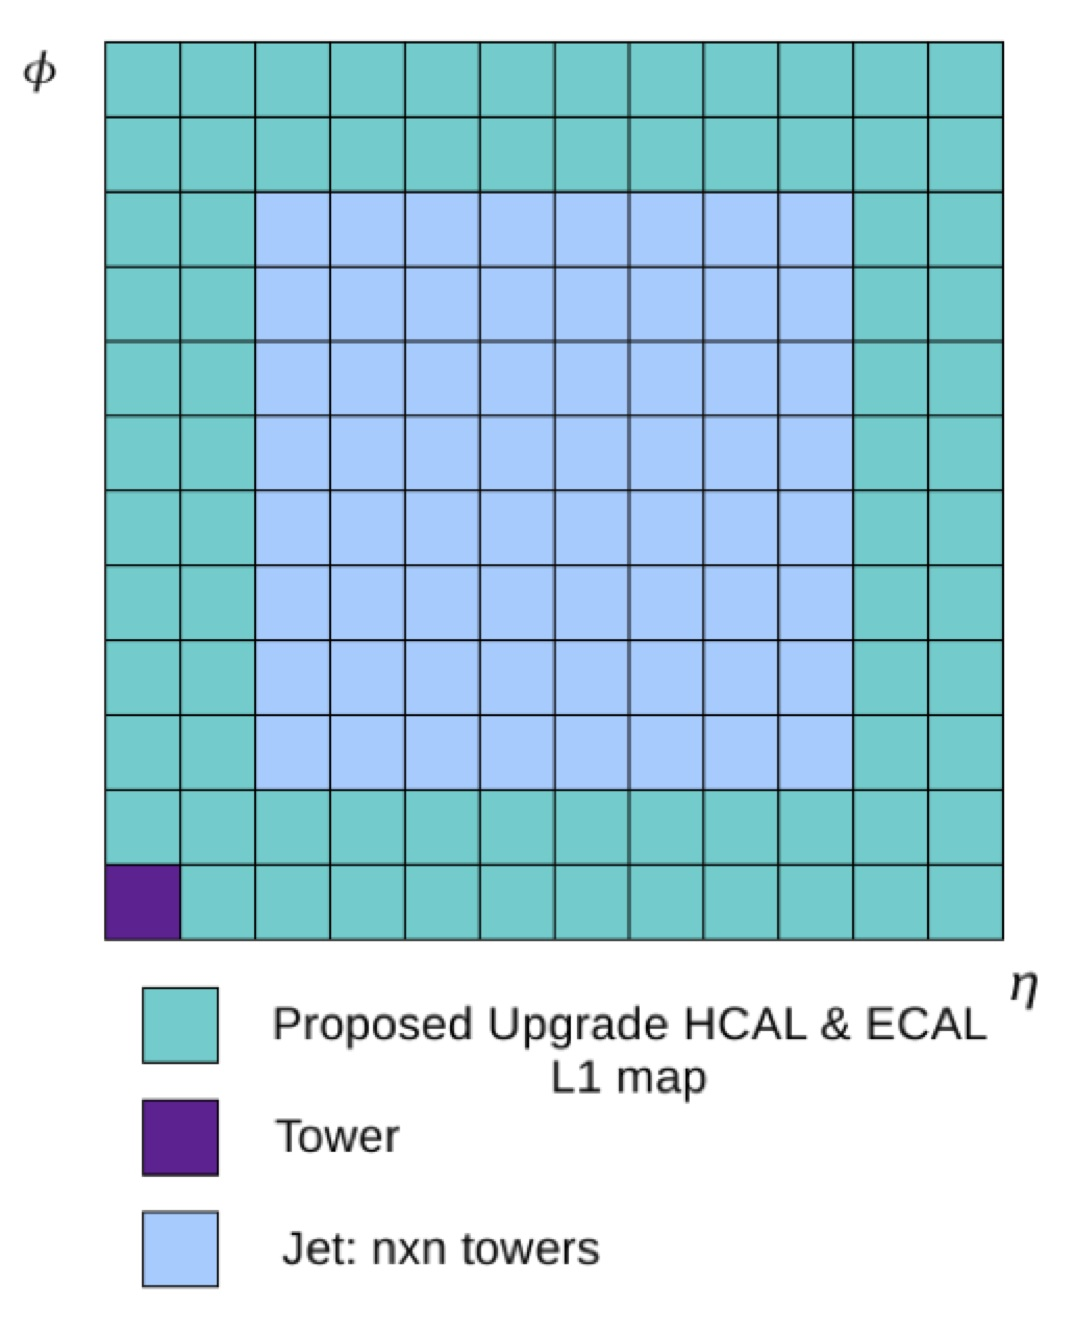
\includegraphics[scale=0.37]{Figures/l1jets/UpgradeJet.jpg} 
\caption{Comparison of the current \ac{L1} jet map, left, with the proposed upgrade jet map, showing a $8\times8$ square jet, right.}
\label{fig:jetcartoon}
\end{center}
\end{figure}


A candidate is created at each individual tower, using a ``sliding window'' approach. 
Only jet candidates with non-zero energies are passed onto the next stage, 
however there remains a huge jet multiplicity at this first stage of jet creation. 
There is a jet for every non-zero tower, and a huge number of overlapping jets as each tower contributes to $n^{2}$ different jets, or, equivalently, each jet candidate has $(2n - 1)^{2}$ overlapping jets.
Figure~\ref{slide} shows some of the jet candidates which overlap, shown in red, with a single jet candidate measuring $4\times4$ towers and square in shape, shown in purple.
The window of all overlapping candidates is shown in blue; and measures $10\times10$ towers.
The resulting numerous overlapping jets must be sorted and filtered to find the highest energy jet of the candidates.

\begin{figure}[ht!]
%\vspace{-1.cm}
\begin{center}
%  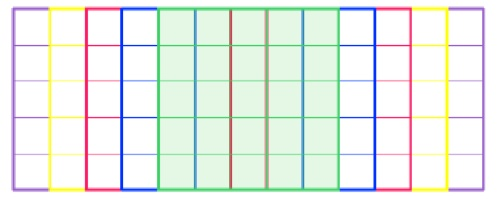
\includegraphics[scale=0.37]{Figures/l1jets/JetOverlaps.jpg}
  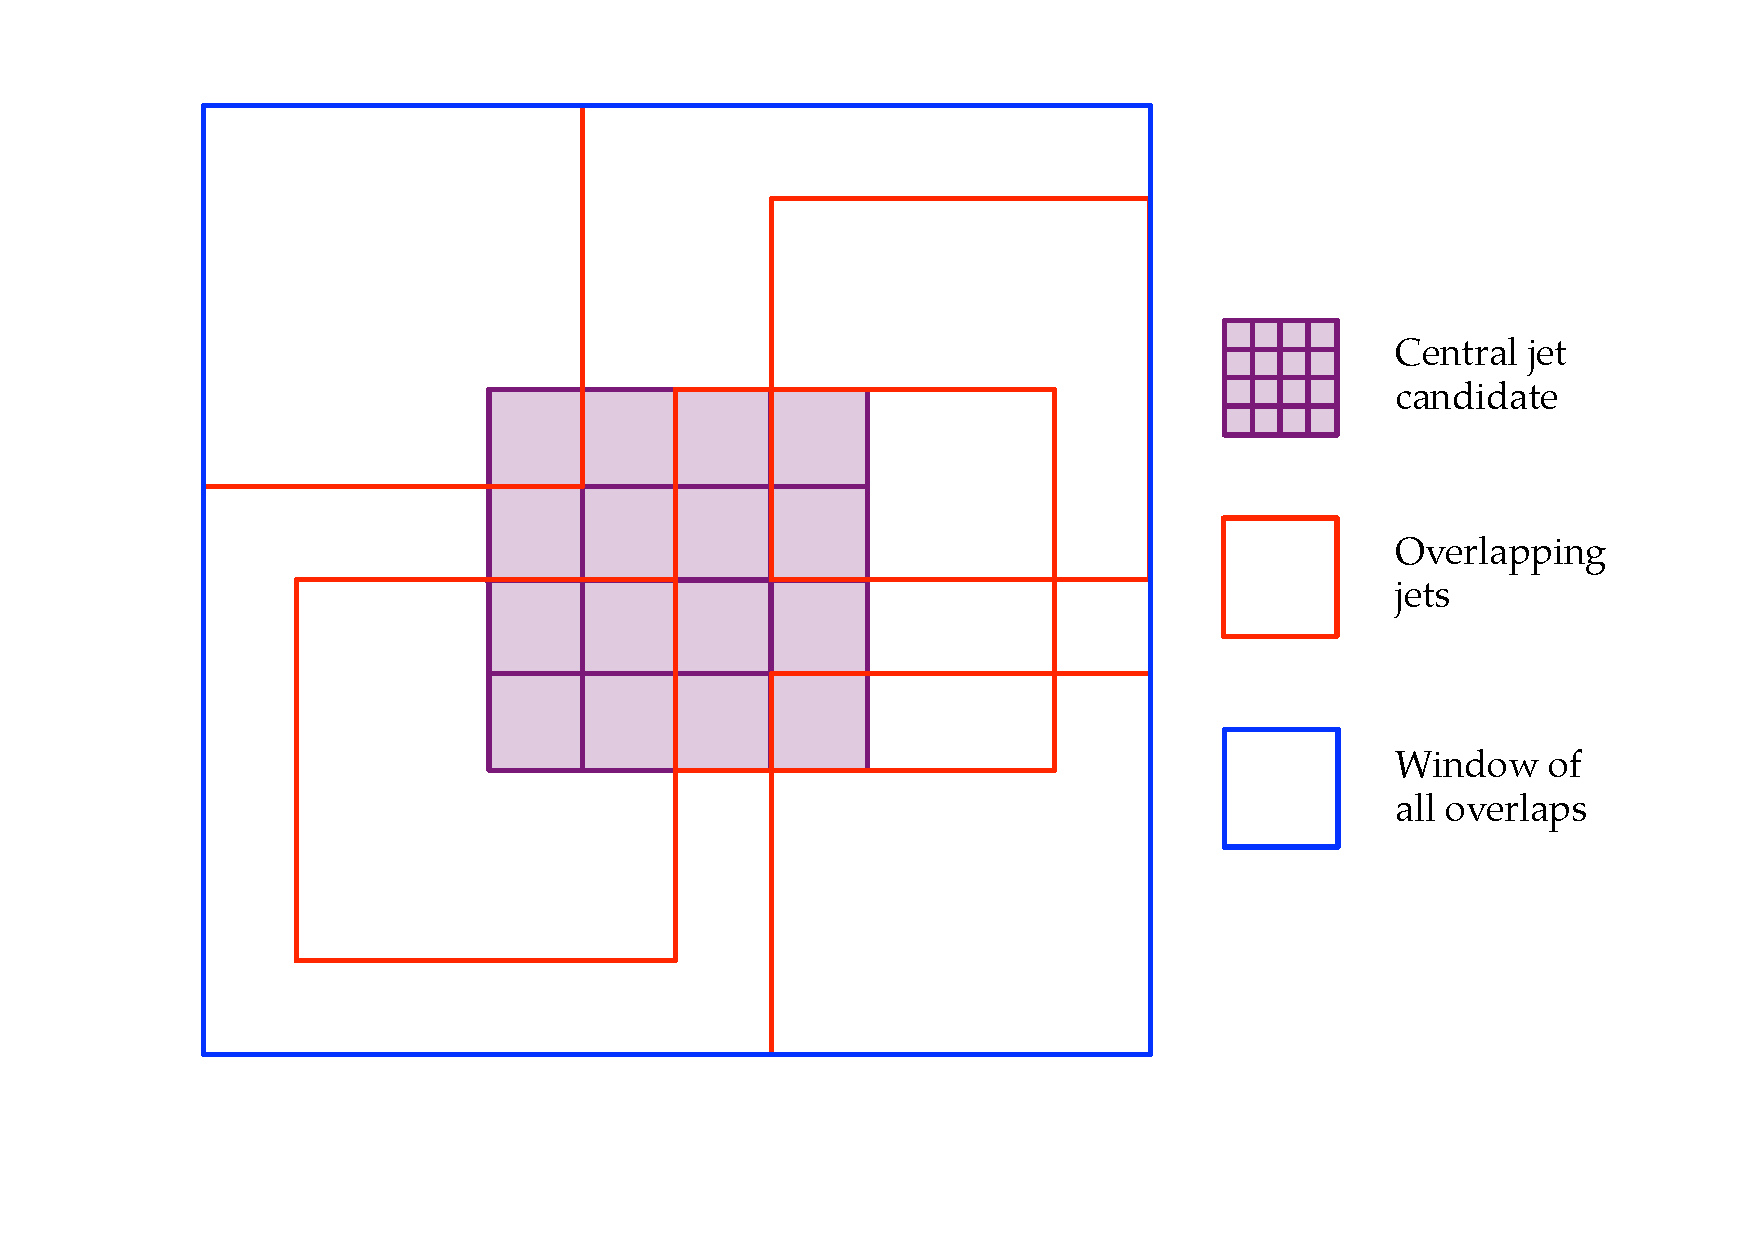
\includegraphics[scale=0.37]{Figures/l1jets/jetoverlaps}
\caption{A few of the overlapping jets of one $4\times4$ jet (centre, purple), are shown in red. The window of all of the jet overlaps is shown in blue, measuring $10\times10$. These overlapping jets must be sorted and filtered to keep only the most energetic jet.}
\label{slide}
\end{center}
\end{figure}

To give the best angular resolution, the $\eta$ and $\phi$ coordinates of the jets are energy weighted,
\begin{eqnarray}
\eta_{jet} &=& \frac{\sum{\eta_{\rm tower} \cdot E_{\rm tower}} } {\sum{ E_{\rm tower} } }  \\
\phi_{jet} &=& \frac{\sum{\phi_{\rm tower} \cdot E_{\rm tower}} } {\sum{ E_{\rm tower} } } . 
\end{eqnarray}
Here, the sum is over all of the towers in a jet window and $\eta_{\rm tower}$, $\phi_{\rm tower}$ are the coordinates of the individual towers within a jet, $E_{\rm tower}$ is the transverse energy deposit in the tower and $\eta_{jet}, \phi_{jet}$ are the coordinates of the jet.


In \added{my} previous studies diameter 8 circular jets, because they are smallest, gave the best angular resolution, so these are presented here. 



\subsection{Jet filtering} 
The jet collection must be sorted and filtered to remove the numerous overlaps.
Firstly, all jets in each event are ordered in energy using a bitonic sort.
This is a recursive parallel sorting algorithm suitable for implementation in hardware.
It takes $2^N$ inputs and sorts in $N$ steps using a series of bitonic sequences and splits.

However, there is often more than one overlapping jet of a particular energy. 
An asymmetry parameter in $\eta$ and $\phi$ is also considered for each jet when this is the case:
\begin{equation}
 \begin{split}
 A_{\eta, \phi} = & \sum \left( \text{Constituent tower energies in positive } \eta , \phi \right) \\ & - \sum \left( \text{Constituent tower energies in negative } \eta, \phi \right) ,
 \end{split}
\label{eqn:Asym}
\end{equation}
\added{
where positive and negative values are defined with respect to the jet centre.
}
A jet with all of its energy in the central tower will have $A_{\eta, \phi} = 0$ 
whereas a jet of the same energy with all energy deposits in an outer tower
 will have large $|A_{\eta, \phi}|$. 
If overlapping jets have the same energy, they are instead sorted 
to give the lowest asymmetry parameter.
The first element in the sorted list is then the most energetic jet, with its energy concentrated most centrally within the $n\times n$ window.

 The sorted list is then filtered to remove jets which overlap with this first jet.
 The process is repeated until 13 separate jets are found. 
 This number is somewhat arbitrary, and is limited by hardware at some high number.
 
Jets are sorted initially in one dimension, along $\eta$ or $\phi$, and overlaps in one dimension are removed. 
The resulting list of the most energetic jets along or around the calorimeter is then sorted in the other direction to give the final jet collection.


\subsection{Event-by-event estimation of pile-up} 

The measurement of the PU contribution to the jet energy 
is evaluated event by event using a method inspired by the paper of 
Cacciari and Salam~\cite{rho_jetarea} and already used to correct offline jets.
In a pp collision with a large number of overlapping proton-proton interactions, 
a large number of relatively soft jets originate from PU and are distributed roughly 
evenly across the calorimeter.  
The median jet transverse energy is therefore very likely to come from PU \added{and the underlying event}, and gives a good estimate of the typical transverse energy of a \ac{PU} jet in the event.
Further, the energy density of the median jet transverse energy gives a good estimation of the energy density due to \ac{PU} across the calorimeter.
The energy released by \ac{PU} per unit area in each event, denoted by $\rho$, can therefore be estimated using the median jet transverse energy, and the area of the jet:
\begin{eqnarray}
 \rho^{\rm L1} &=& \frac{ \langle E^{\text{L1 jet}}_{\rm T} \rangle }{A_{\text{L1 jet}}}
\end{eqnarray}
where $\langle E^{\text{L1 jet}}_{\rm T} \rangle$ denotes the median jet transverse energy, and $A_{\text{L1 jet}}$ denotes the jet area.
The energy of all jets in an event can then be corrected for the energy density due to \ac{PU} \added{and the underlying event} by
simply subtracting from all jets in an event using
\begin{eqnarray}
 \text{PU corrected }E_{T} &=& E_{T} - \rho^{\rm L1} \times A_{\text{L1 jet}} ,
 \label{eqn:PUsub}
\end{eqnarray}
because the energy density due to \ac{PU} across the calorimeter is assumed to be uniform. 
This assumption is valid for \ac{PU} values of order $\sim50$, however as \ac{PU} increases above 100 pp collisions in each bunch crossing, simulation shows many more soft \ac{PU} jets are expected to lie in the forward regions of the detector, so an $\eta$ dependent \ac{PU} subtraction may be more suitable for very high \ac{PU} scenarios.
This is not investigated here, but is within the capabilities of the upgraded trigger system.

In the following we show the effect of PU subtraction in the measurement of the
jet energy. The same quantity could also be used to correct the contribution of \ac{PU} to quantities used to define electrons/photons; isolation parameters, and the ratio of transverse energy deposits in the \ac{HCAL} and \ac{ECAL}.


\subsection{Calibration to the jet energy scale \label{jet_calib}}

\added{
Different regions of the detector do not necessarily give the same 
response to an incoming jet. Certain regions may be less-well instrumented, and produce an energy measurement that is smaller than a more highly instrumented region would give to the same jet, for example. 
}
The raw jet energies from the calorimeter towers must be corrected to the jet energy scale 
\added{
in order to take into account this effect.
}\deleted{Different regions of the calorimeter give different responses so} 
A set of calibration constants 
in \pt and $\eta$ are \added{therefore} derived, \added{in order to provide a look-up table to be used online, so that energy deposits can be calibrated to the jet energy scale in real time}. %: so-called "L2L3 corrections".

A non linear regression method is used on an independent \replaced{sample}{subsection} of 
20,000 events collected using a single muon trigger. Events which contain a least one muon often have hadronic activity in the opposite hemisphere to the muon and so the data sample provides a sufficient number of jets to do a statistically meaningful calibration. 
\added{This sample of events is subsequently removed from data sets used to characterize performance of the algorithm in the following sections: they are statistically independent.}

Once the \ac{L1} upgrade jets have been created, sorted and filtered, the value of the average energy density due to \ac{PU}, $\rho^{\rm L1}$, 
\added{which is calculated on an event-by-event basis,} 
is calibrated to the jet energy scale by comparing it \added{to a lookup table of $\rho$ values, created by comparing the online $\rho$ with that calculated offline for each event in an independent sample}.
The corrected \ac{PU} subtraction parameter is applied to the \ac{L1} jets in the event according to Equation~\ref{eqn:PUsub}, in order that they 
can be calibrated to the offline jets which have been similarly \ac{PU} subtracted.
The leading offline jet in each event, where the jet is formed using the anti-k$_{\rm t}$ algorithm with radius parameter of 0.5 and inputs from the calorimeter alone, ``AK5 Calo jets'', is matched to a L1 jet within a cone of 
$\Delta R = \sqrt{ (\eta_{L1} - \eta_{offline})^2 + (\phi_{L1} - \phi_{offline})^2} < 0.5$.
The use of AK5 Calo jets\added{, rather than AK5 PF jets,} gives reconstructed offline jets as close as possible to those created at \ac{L1}, as both are built using calorimeter information alone.
The values of \pt and $\eta$ for the matched \ac{L1} and offline jets are used as inputs to a multi-variate analysis.  
This provides a lookup table of multiplication factors binned in values of the L1 jet $\eta$ and $\pt$. 
Applying this calibration to the \ac{L1} jets gives a calibration independent of PU. 

The distribution of L1 jet \pt, where each jet has been matched to an offline jet, before and after the calibration has been applied is shown in Figure~\ref{prepostCalib}. 
Momenta are much more closely matched after the calibration has been applied.

\begin{figure}[t!]
\begin{center}
  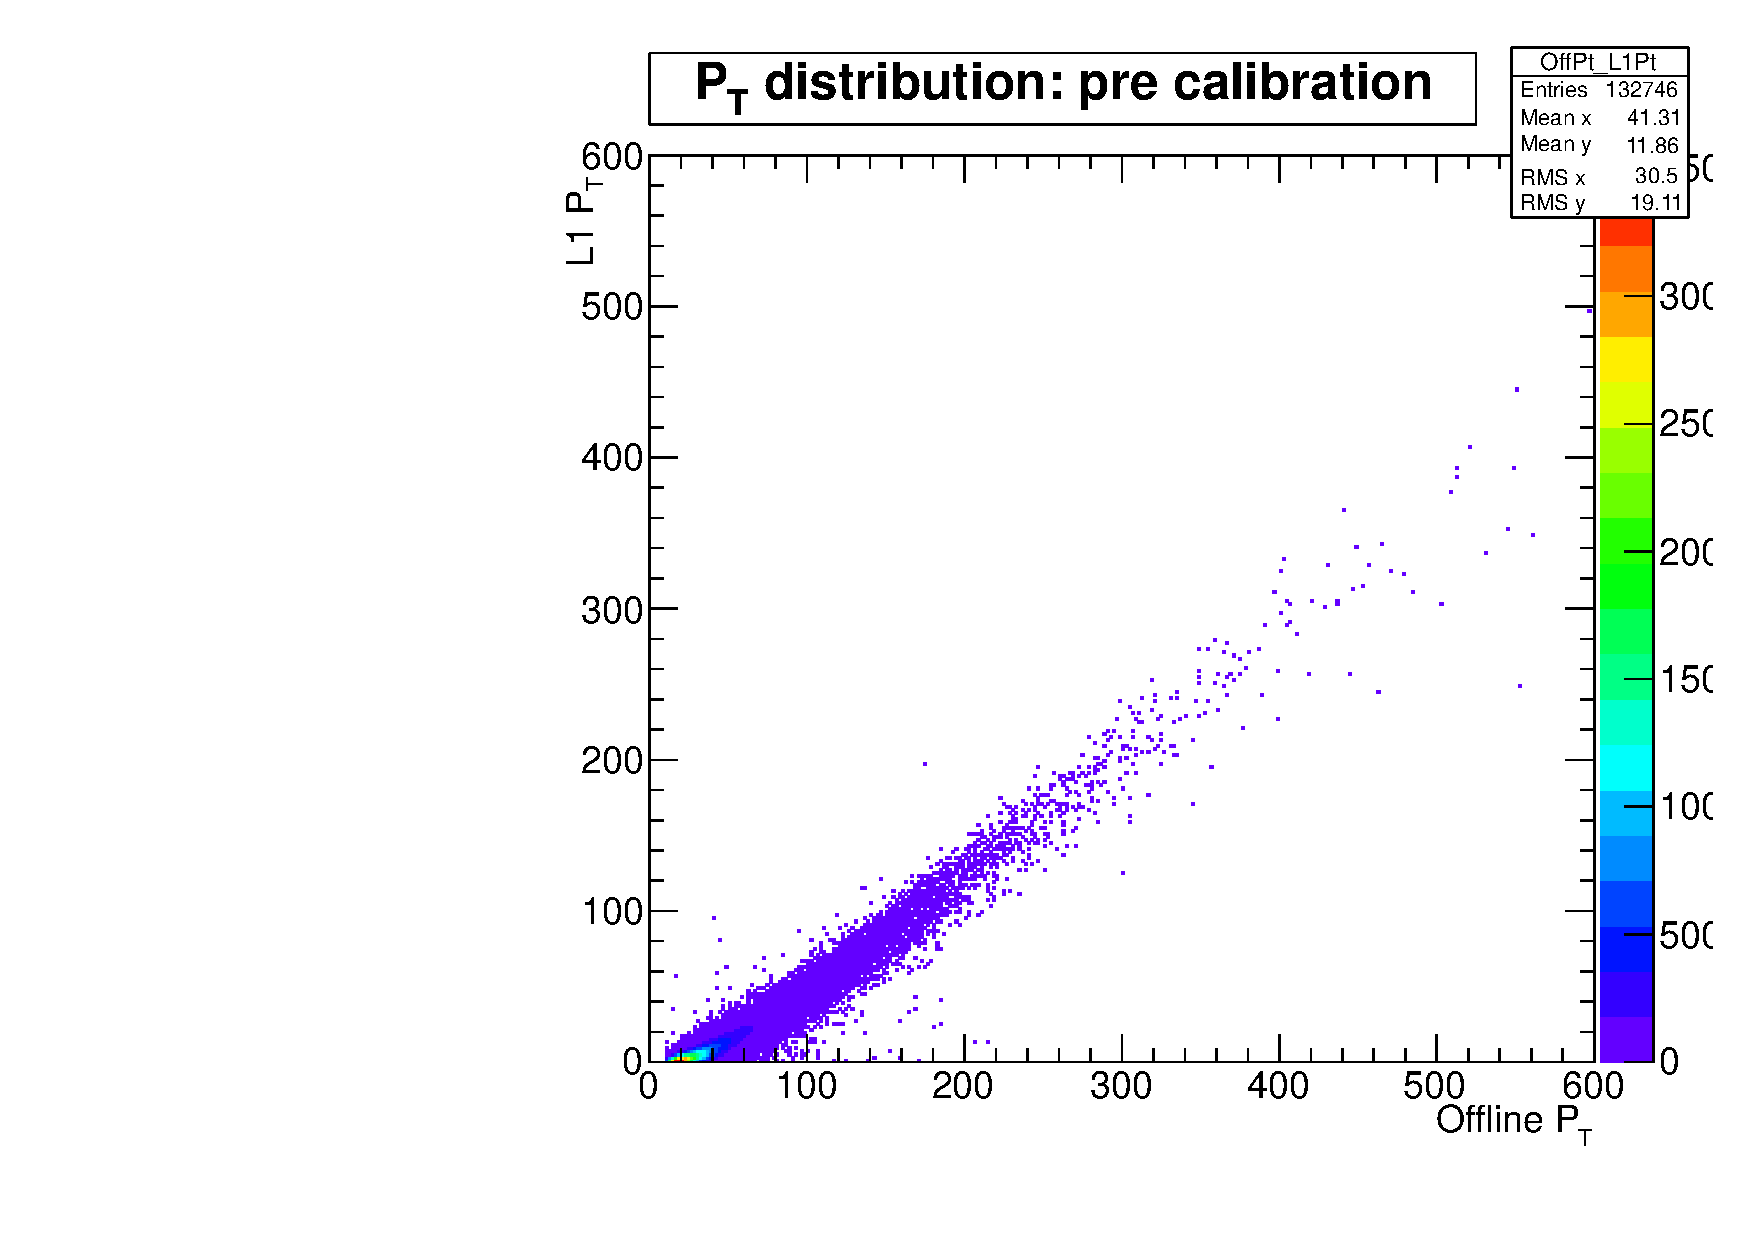
\includegraphics[scale=0.32]{Figures/l1jets/PreCalib.pdf}
  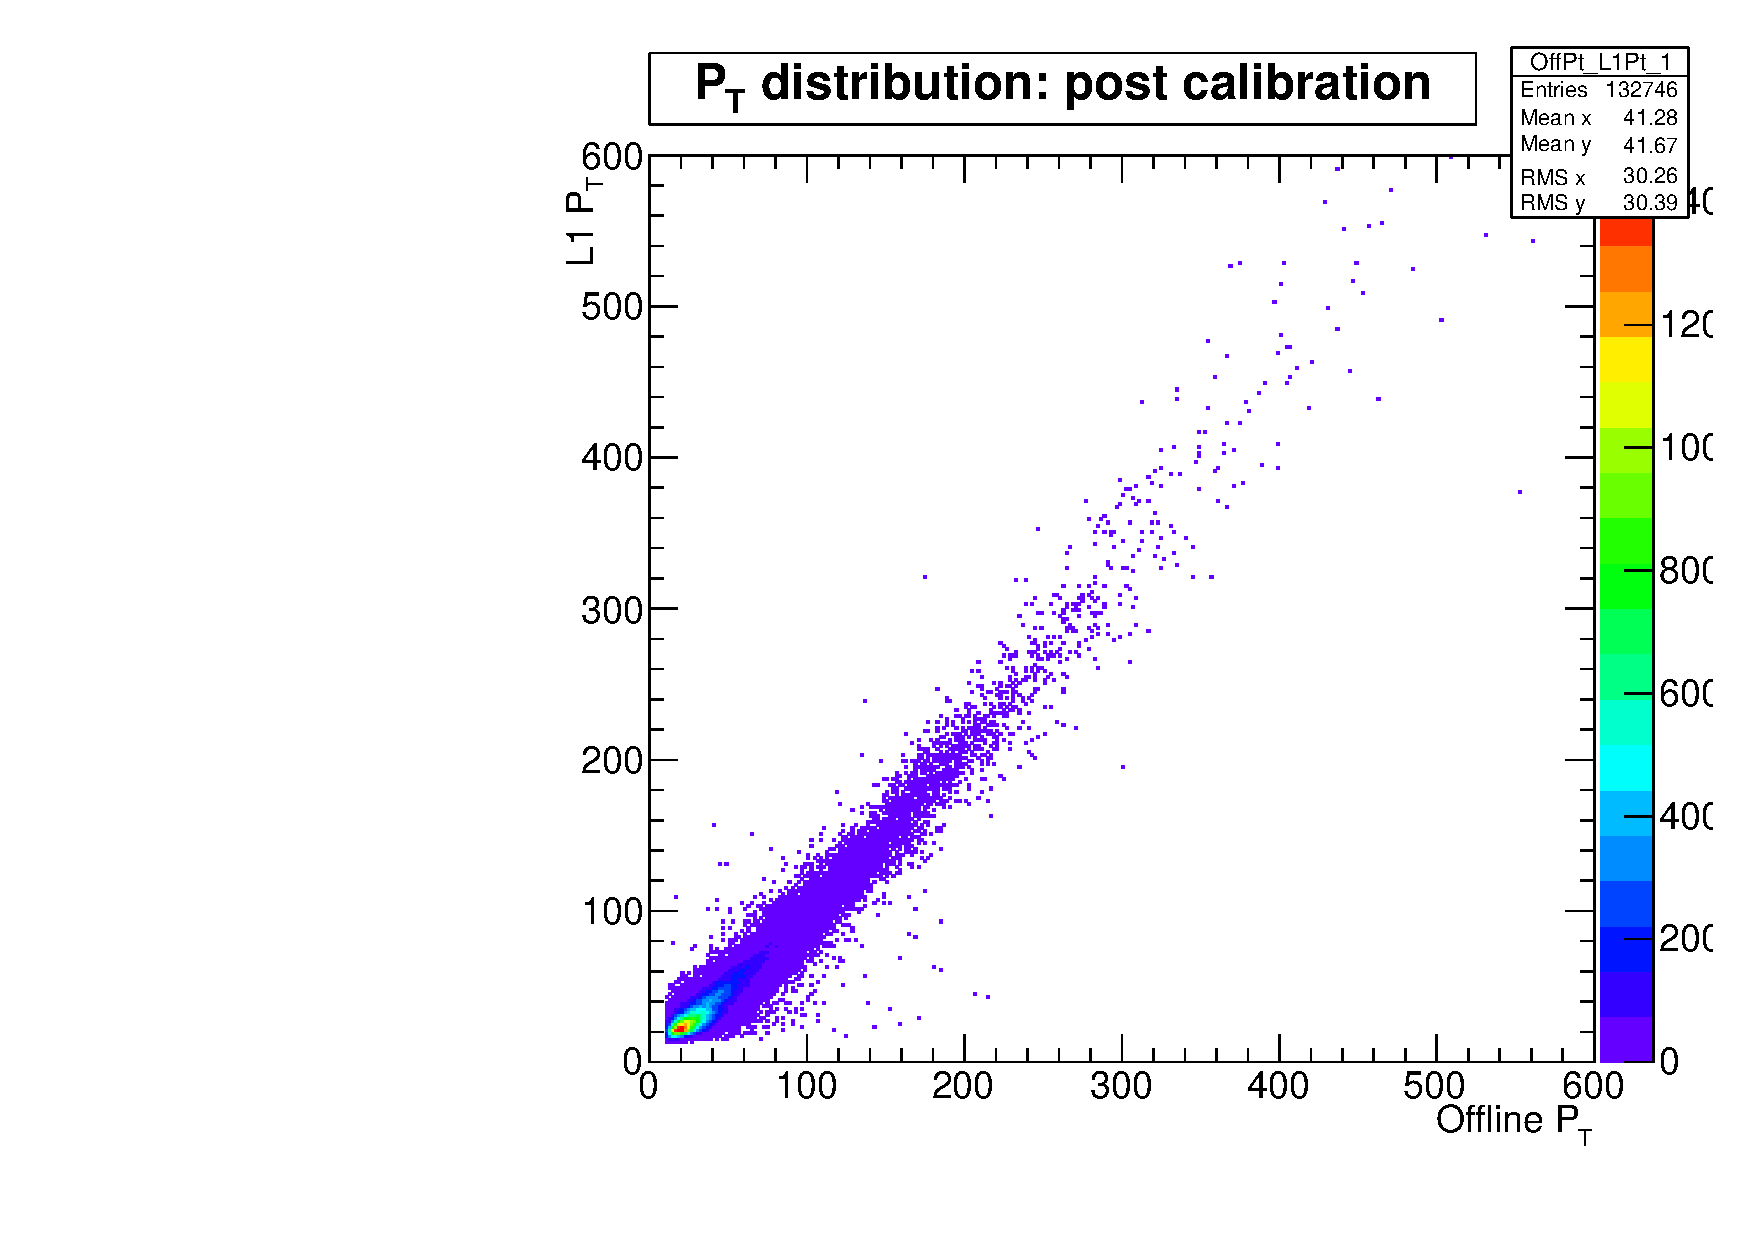
\includegraphics[scale=0.32]{Figures/l1jets/PostCalib.pdf}
\caption{The \pt distribution of \ac{L1} jets that have been matched, within a cone of $\Delta R<0.5$, to offline jets reconstructed with the anti-k$_{\rm t}$ algorithm using a radius parameter of 0.5 and calorimeter information as input only. The distribution shown before a \pt and $\eta$ calibration has been applied is shown on the left, and after the calibration has been applied on the right. In both distributions, \ac{PU} has been subtracted from both jet collections. }
\label{prepostCalib}
\end{center}
\end{figure}



\section{Upgrade L1 Jet Algorithm Performance}

Jet performance can be characterised by angular and energy resolutions, efficiency of reconstruction and trigger rates. 
The proposed upgrade \ac{L1} jets were simulated using data that were collected in high \ac{PU} conditions during 2012, where events were selected at random from the whole dataset, for example every $10^{\rm th}$ event kept --- termed ``Zero Bias'' data. 
The \ac{LHC} run used for the study had an average of 45 primary vertices per bunch crossing, \added{and had integrated luminosity of 0.03~pb$^{-1}$}.  

\subsection{Angular and energy resolutions}

Resolutions are measured as compared to offline AK5 Calo jets, as described in Section~\ref{jet_calib}. 
The leading offline jet (which must have $\pt > 20$~\GeV) is matched to a  \ac{L1} jet within $\Delta R < 0.5$, and the resolutions are defined as:
\begin{eqnarray}
\sigma_{\eta} &=& \eta_{offline} - \eta_{L1} \\
\sigma_{\phi} &=& \phi_{offline} - \phi_{L1}\\
\sigma_{\pt} &=& \frac{ \pt^{offline} - \pt^{L1} } { \pt^{offline} } 
%\Delta_{\rho} &=& \frac{\rho_{AK5Calo} - \rho_{L1} } {\rho_{AK5Calo}}
\end{eqnarray}  

Angular and energy resolutions of the proposed upgrade algorithm compared to the current system are shown in Figure \ref{JetRes}.
There is a much improved angular resolution as the upgrade jets take advantage of the full granularity of the calorimeter. 
In high PU data, the energy resolution is improved due to the PU subtraction. 
With the current \ac{L1} jet algorithm, there are a significant number of events in which 
\added{the energy of the \ac{L1} jet has been falsely boosted by \ac{PU}, and it is matched to a relatively soft offline jet, } 
\deleted{the leading offline jet has been matched to low energy \ac{PU} \ac{L1} jets, }
giving a negative value of $\sigma_{\pt}$ and giving rise to the significant negative tail in the distribution.

\begin{figure}[t!]
\begin{center}
  \includegraphics[scale=0.32]{Figures/l1jets//etaRes.pdf}
    \includegraphics[scale=0.32]{Figures/l1jets//phiRes.pdf}
       \includegraphics[scale=0.32]{Figures/l1jets//ptRes.pdf} 
\caption{Resolution in $\eta$, $\phi$ and \pt for high \ac{PU} data taken by the \ac{CMS} detector in 2012. There is a clear improvement with the upgrade jets, plotted in red, in both angular resolutions and energy resolution. These plots can be found in~\cite{Tapper:1556311}.}
\label{JetRes}
\end{center}
\end{figure}

Crucially, the energy resolution of the upgrade jet algorithm shows a much reduced dependence on \ac{PU}, shown in Figure~\ref{JetResPU}.
This is evidence that the event-by-event \ac{PU} subtraction has the intended effect, 
reducing the worsening effect of additional primary vertices on the jet energy resolution, 
and the upgrade jet algorithm is therefore expected to show a reduction in rate compared to the current algorithm.

\begin{figure}[t!]
\begin{center}
  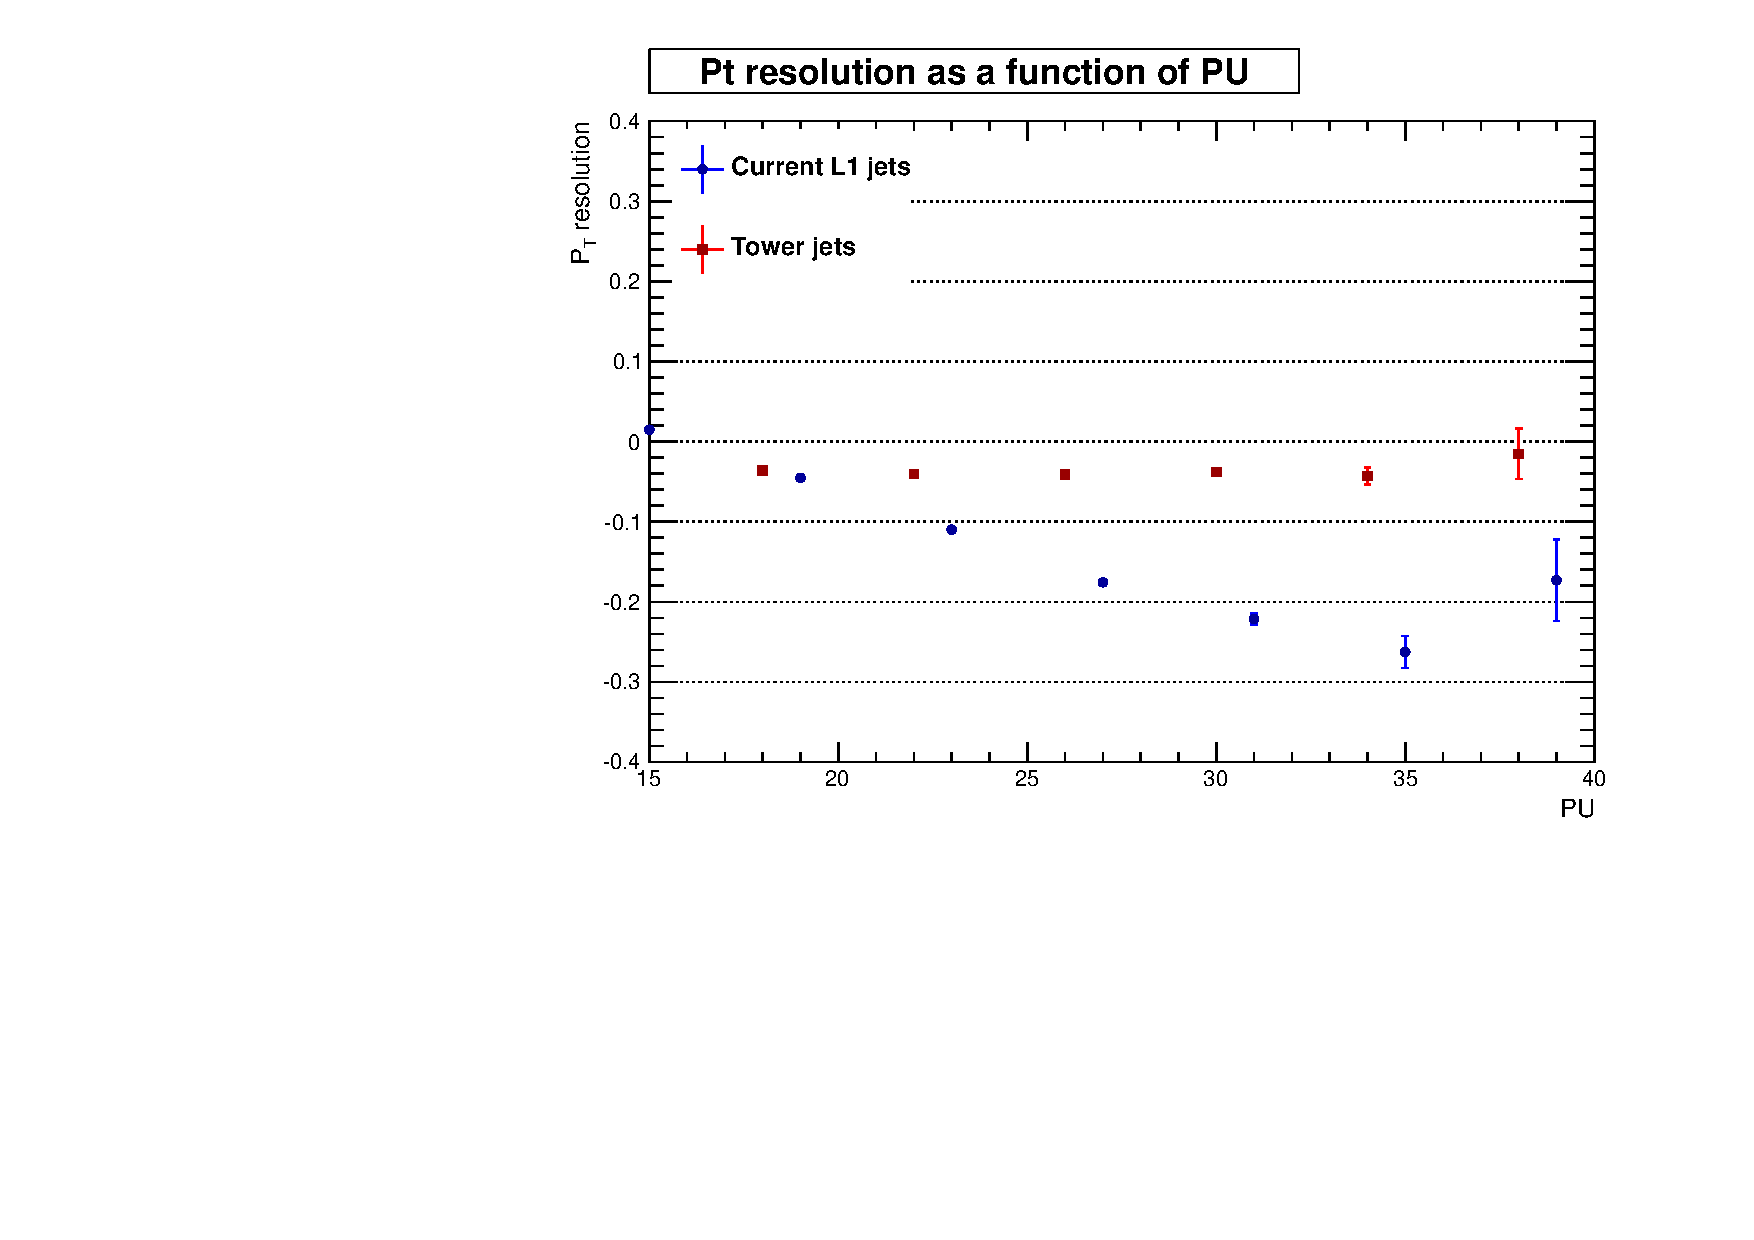
\includegraphics[scale=0.52]{Figures/l1jets/Ptres_vsPU.pdf}
\caption{The \ac{PU} dependency of the \ac{L1} jet energy resolution for both the current algorithm and the upgrade algorithm, where the resolution is taken as the RMS of the PU distribution shown in Figure~\ref{JetRes}, for different \ac{PU} bins. There is a clear improvement with the upgrade jets, plotted in red, which shows independence of \ac{PU} up to \ac{PU}$\sim$40.}
\label{JetResPU}
\end{center}
\end{figure}

\subsection{Trigger efficiencies}
The trigger efficiencies for various \ac{L1} jet transverse energy thresholds are measured, as compared to AK5 Calo jets, to show the effectiveness of the proposed algorithm at reconstructing jets which have been measured offline, which are treated as the ``truth''.
If the leading \ac{L1} jet in each event above a certain energy threshold is matched to an offline jet, the energy of the matched offline jet is plotted. 
All matched offline jet energies are also plotted. 
By taking the ratio between these two distributions we attain trigger turn on curves, shown in Figures~\ref{JetTO_lowPU} and \ref{JetTO_highPU}.

The sharpness of the turn on curve is due to the energy resolution of the jet algorithm.
If all of the \ac{L1} jets have reconstructed energies that exactly equal the energies of the offline jets to which they are matched,
i.e. $\sigma_{\pt} = 0$, there would be a step function at the value of the jet energy threshold of the trigger.
The turn on would be instant at the specified trigger threshold.
%
The plateau efficiency of the turn on is dictated by the matching efficiency of the jet algorithm.
If all \ac{L1} jets are perfectly matched to offline jets then the algorithm is fully efficient at reconstructing jets at \ac{L1} and the plateau efficiency is 1.

The turn on curves shown in Figure~\ref{JetTO_lowPU} are taken from data taken using the same single muon trigger as was used for the jet calibration, where the presence of at least one muon in each event implies there is often hadronic activity in the opposite hemisphere of the detector to the muon. 
This is a relatively low \ac{PU} set of events, with approximately 20 pp interactions per bunch crossing. 
\added{
While the plateau efficiency for both algorithms is 1, as you would expect, there is a slightly slower turn-on for the upgrade algorithm -- it does worse than the current algorithm. 
This is down to non-optimal calibration, and could be improved with a better method and more statistics with which to perform the calibration (particularly for high momentum jets). However, it is in the high \ac{PU} data where the improvement can be seen. 
}

Figure~\ref{JetTO_highPU} shows the performance at \ac{PU} of approximately 45, a data sample which has lower statistical precision, hence the larger error bars.
The sizeable negative tail shown in the momentum resolution for the current algorithm in Figure~\ref{JetRes} is 
evident in the bump at low momentum in the left hand plot.
\added{
Relatively soft jets due to \ac{PU} have been falsely boosted, and are reconstructed using the current L1 algorithm to be above the \ac{L1} threshold. 
These are then matched to very soft \ac{PU} jets, reconstructed offline, causing the behaviour at low \pt where many L1 jets are over the L1 threshold, whereas their offline counterparts are not.}
Because the effect of \ac{PU} has effectively been removed from the upgrade \ac{L1} jet collection, this is not the case for the upgrade trigger turn ons. 



\begin{figure}[t!]
\begin{center}
  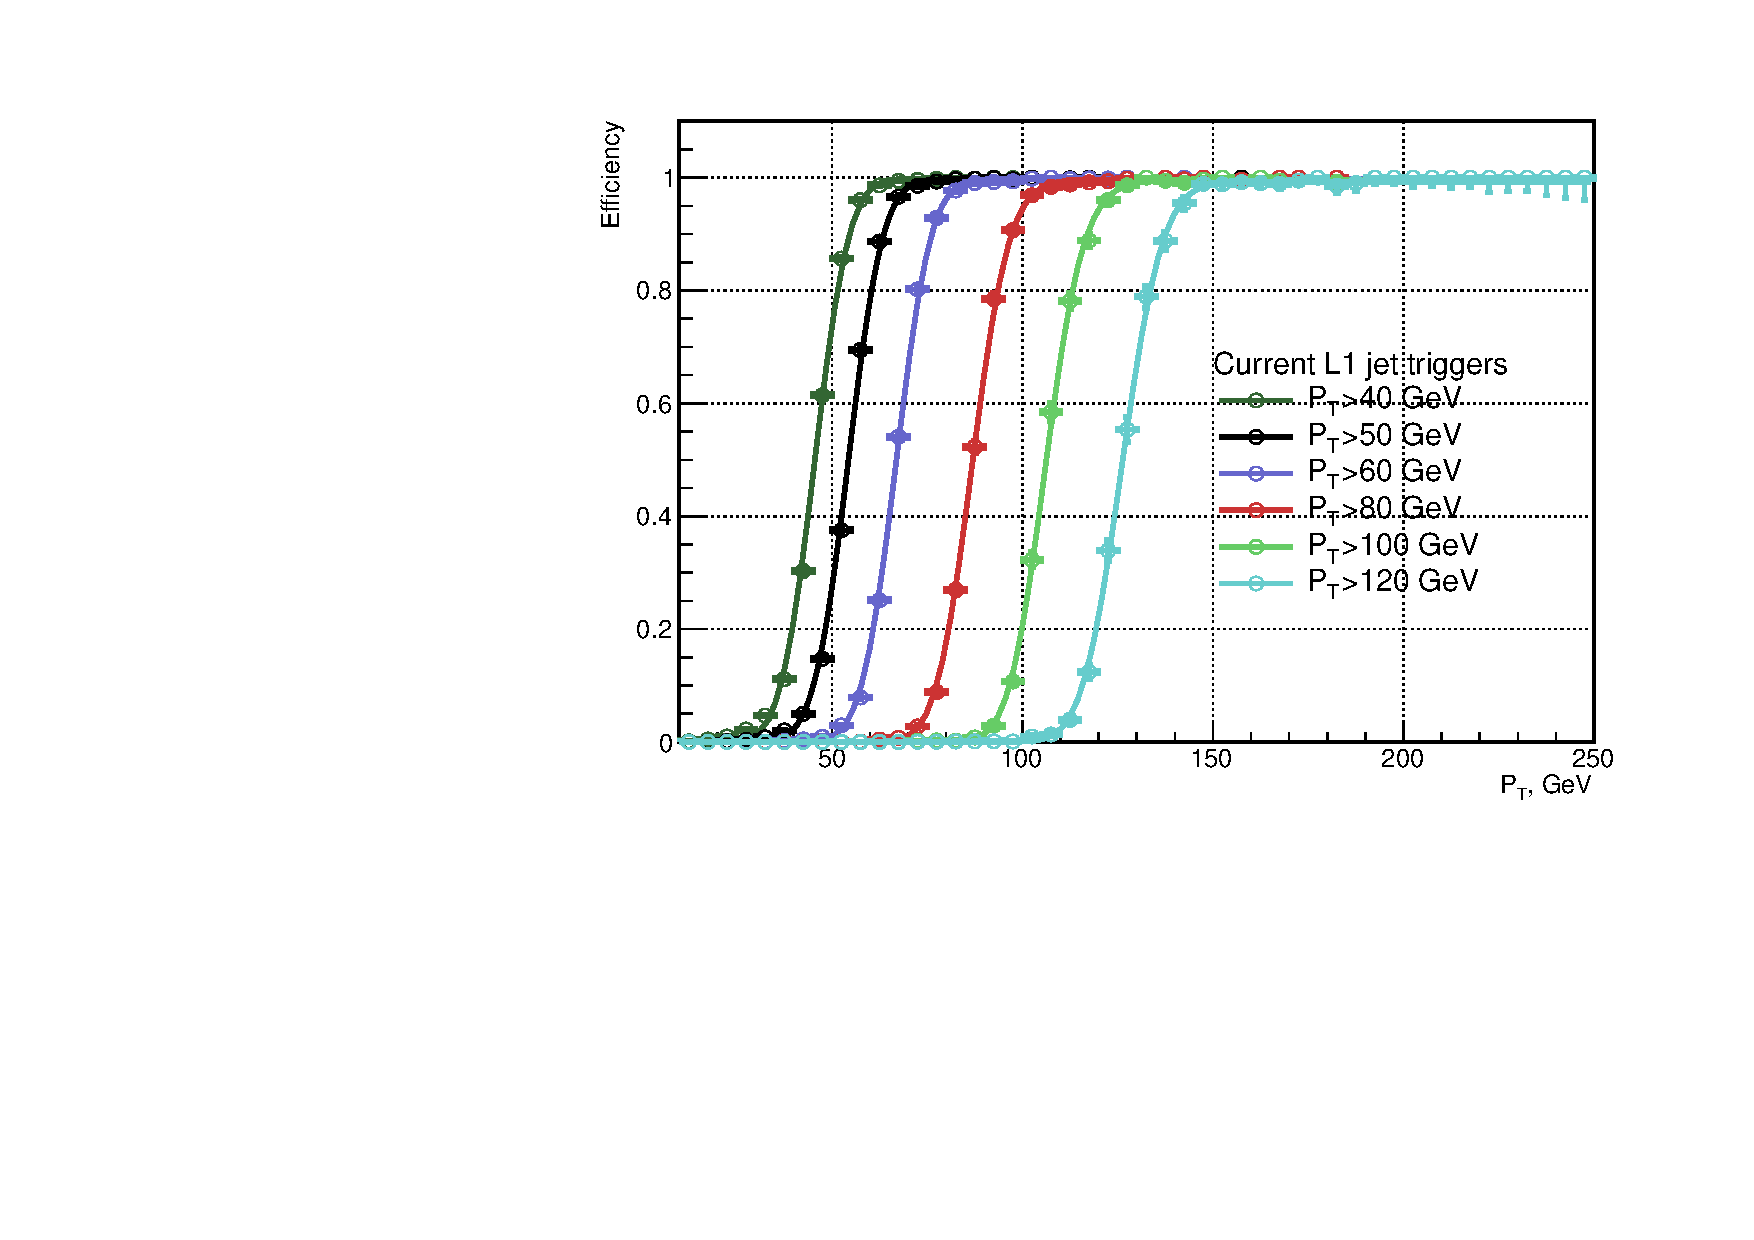
\includegraphics[scale=0.37]{Figures/l1jets//CurrentL1JetTriggers.pdf}
    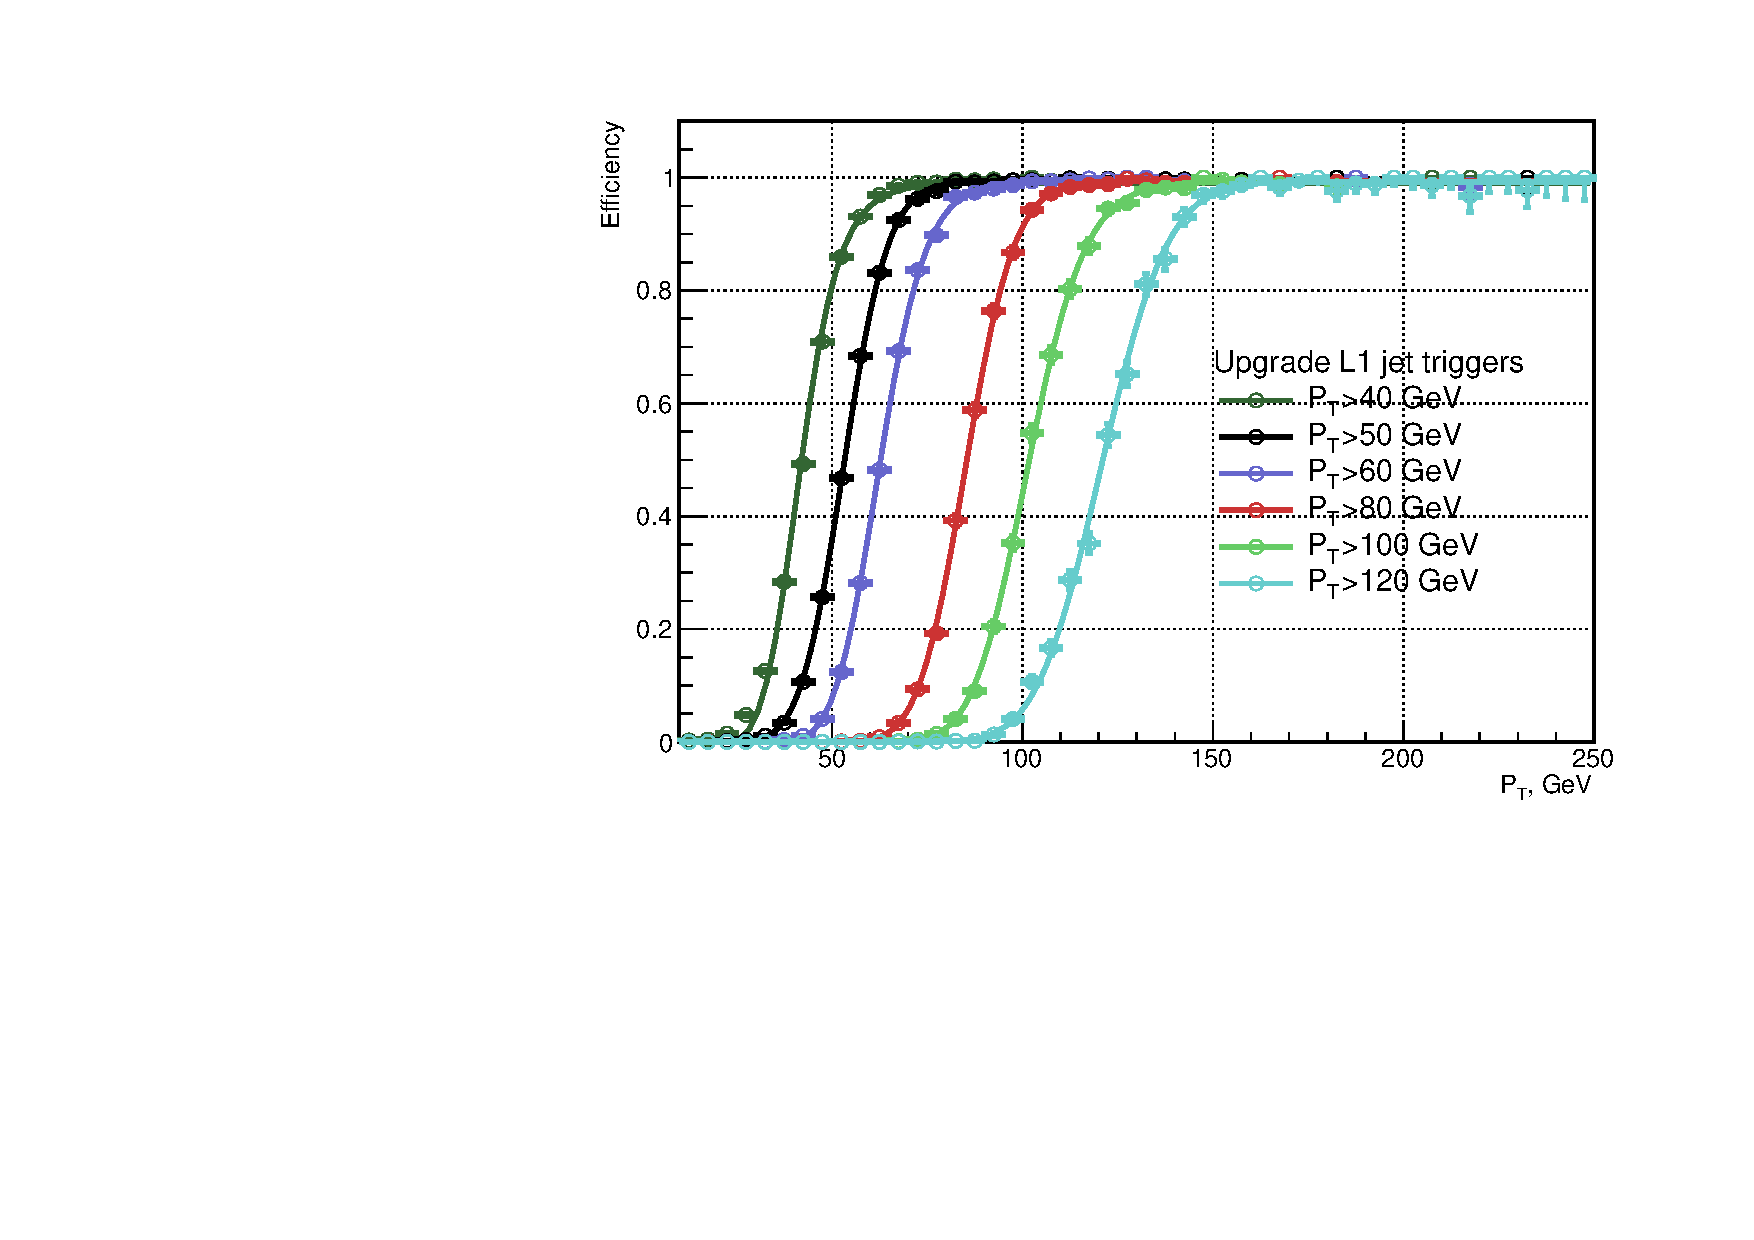
\includegraphics[scale=0.37]{Figures/l1jets//UpgradeL1JetTriggers.pdf}
\caption{On the left are the trigger turn on curves for the current jet algorithm and on the right are the trigger turn on curves for the upgrade jet algorithm, for various single jet trigger thresholds, calculated using relatively low \ac{PU} data. The right hand plot can be found in~\cite{Tapper:1556311}.}
\label{JetTO_lowPU}
\end{center}
\end{figure}

\begin{figure}[t!]
\begin{center}
  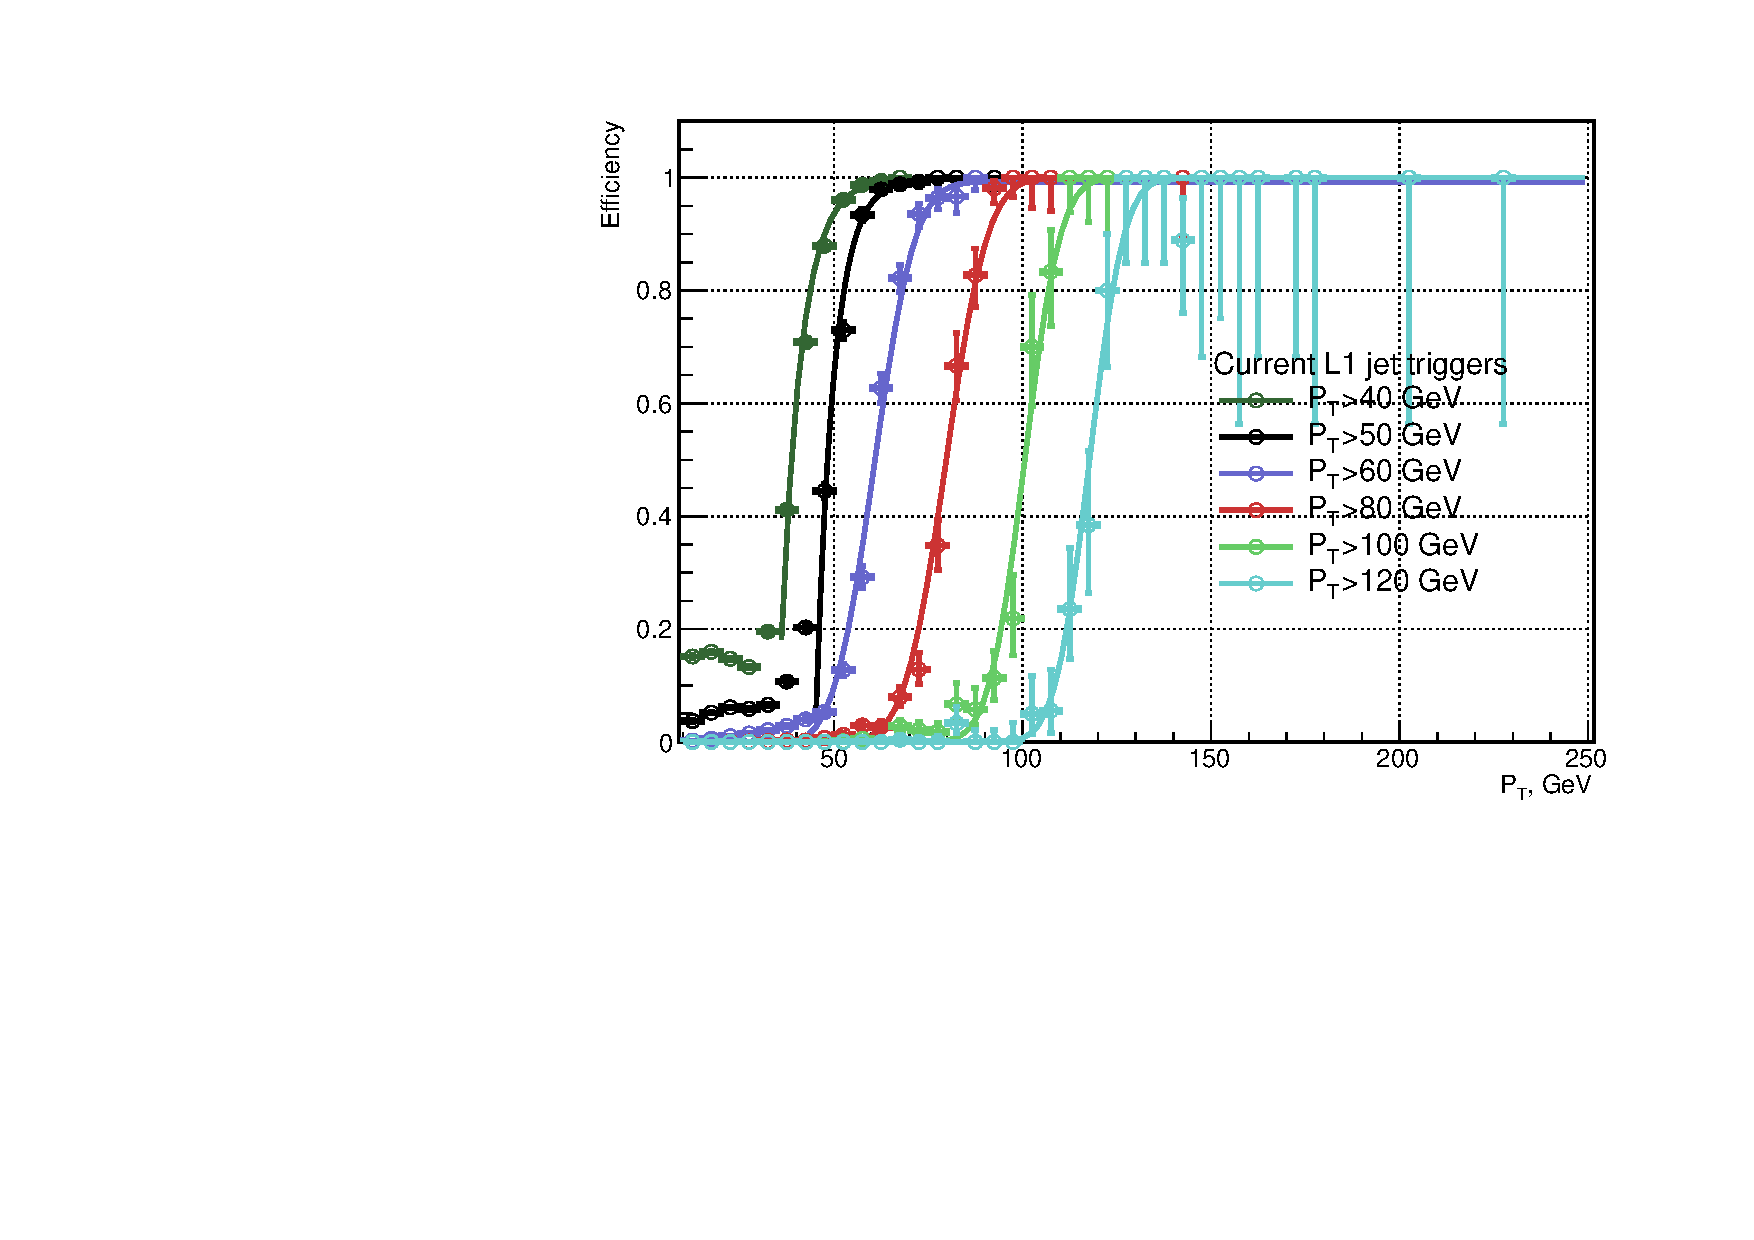
\includegraphics[scale=0.37]{Figures/l1jets//CurrentL1JetTriggersHPU.pdf}
    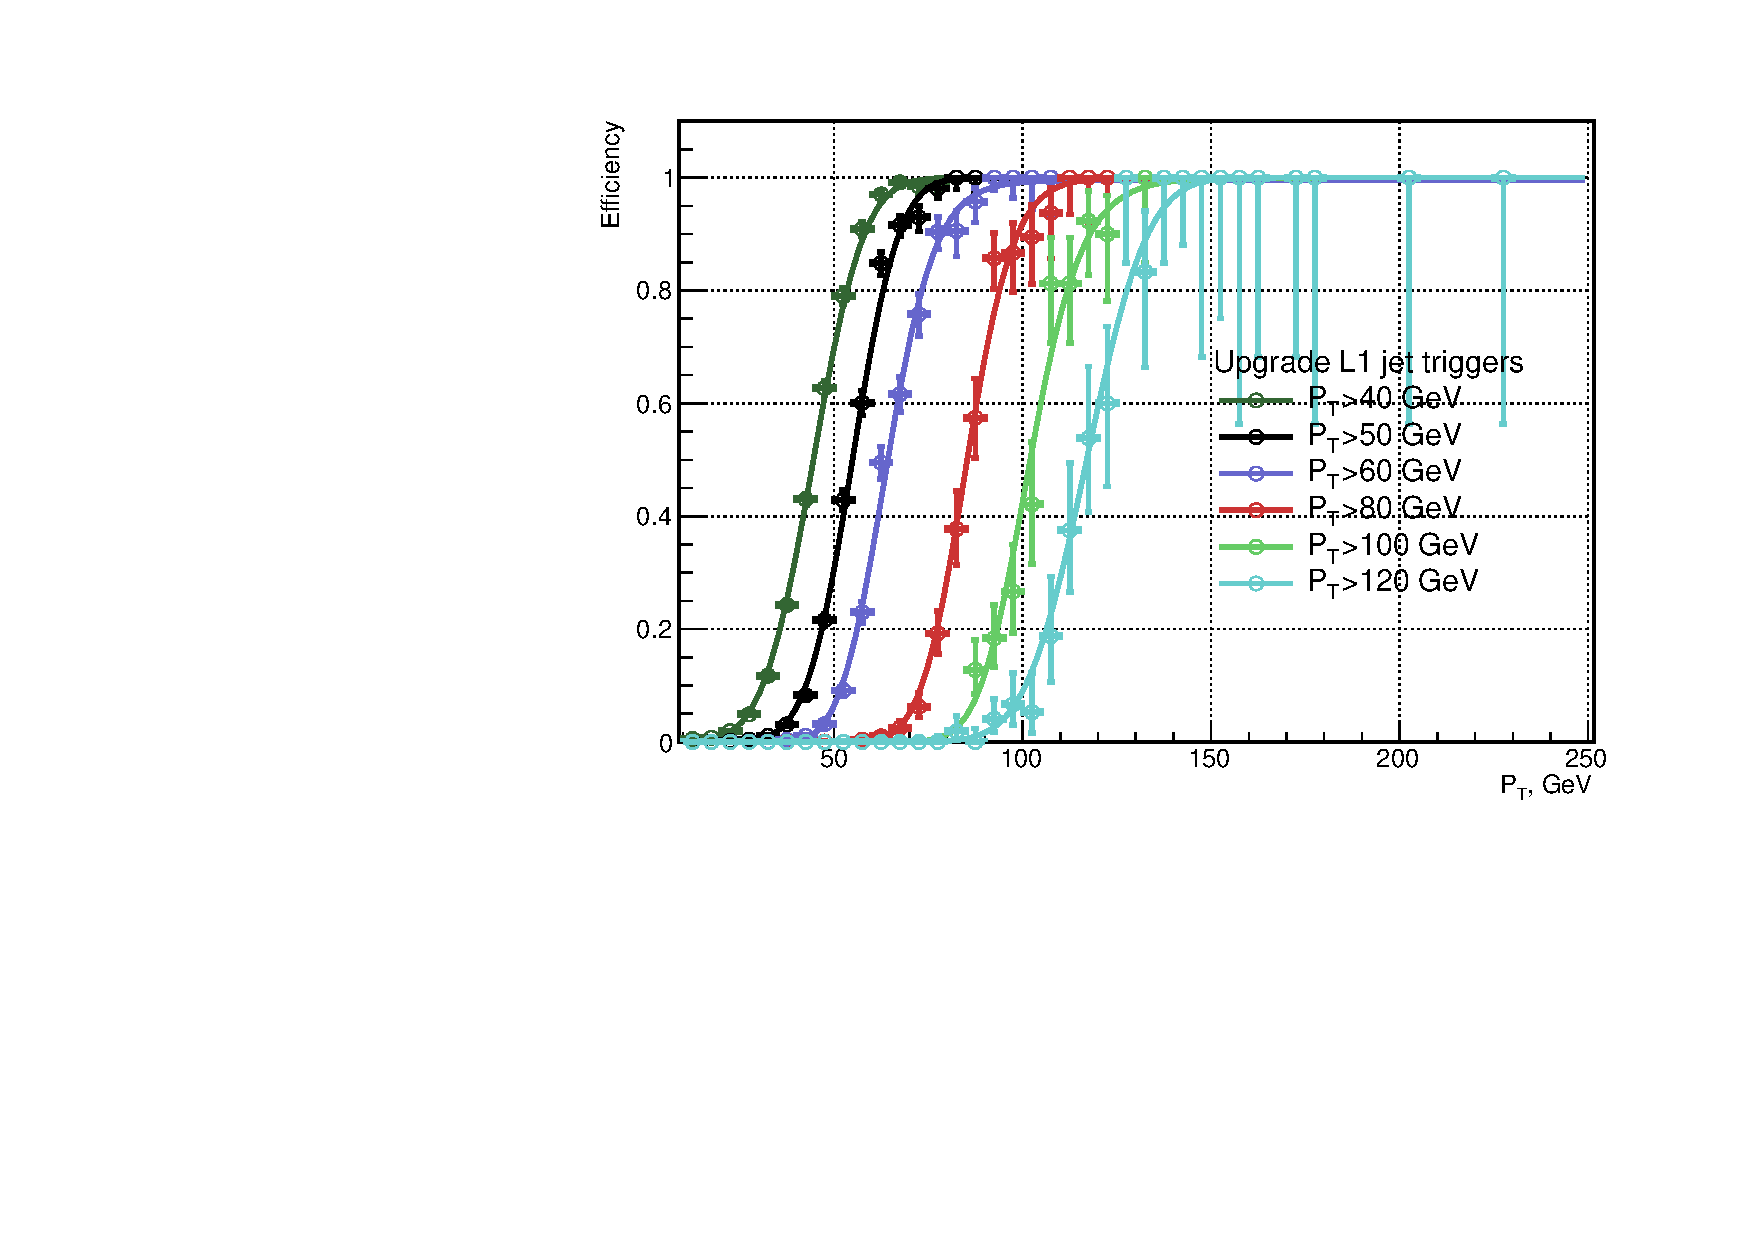
\includegraphics[scale=0.37]{Figures/l1jets//UpgradeL1JetTriggersHPU.pdf}
\caption{On the left are the trigger turn on curves for the current jet algorithm and on the right are the trigger turn on curves for the upgrade jet algorithm, for various single jet trigger thresholds, using relatively high \ac{PU} data.}
\label{JetTO_highPU}
\end{center}
\end{figure}

The \ac{PU} subtraction of the proposed upgrade algorithm is also evident in the upward shift in energy of the turn on curves, going from the current algorithm to the upgrade algorithm;
\added{the sharper turn ons for the current algorithm are now because the \ac{L1} jet energy is falsely boosted by \ac{PU}.}
For a requirement of, for example, one 40~\GeV jet at \ac{L1}, the offline value at which 95\% of events pass the 
trigger is 51.4~\GeV for the current algorithm in the high \ac{PU} dataset; and 62~\GeV for the upgrade algorithm.
Table~\ref{tab:trigTO} shows the offline transverse momentum value at which the trigger is 95\% efficient for the various turn on curves shown in Figure~\ref{JetTO_highPU}.
A lower typical hadronic energy at \ac{L1} in events reconstructed using the upgrade algorithm, 
due to the \ac{PU} subtraction, drives the 95\% efficiency values up. 
\added{While for offline analysis variables to stay as low as possible we ideally want the 95\% efficiency values to be as low as possible, we also want to maintain a low rate. 
With the current algorithm, we will be allowing many more events to pass the threshold, increasing the rate the trigger fires. 
Further, the energy values are falsely high, so the fake rate of events that don't actually contain a jet above threshold will also be high; this is a `waste' of bandwidth as these events will be discarded in offline analysis. }
Plateau efficiency values are 1 in both algorithms, meaning the upgrade jet algorithm (like the current algorithm) is fully efficient at large jet \pt values.

\begin{table}[htb]   
    \begin{center}
        \caption{The 95\% efficiency values for various \ac{L1} jet transverse momentum thresholds, in~\GeV, and plateau efficiency values for the current and upgrade algorithm, for turn on curves taken in high \ac{PU} data and shown in Figure~\ref{JetTO_highPU}.}\label{tab:trigTO}
        {%\small
            \begin{tabular}{c|cc|cc} 
            %\hline
 &   \multicolumn{2}{c|}{Current L1} &  \multicolumn{2}{c}{Upgrade L1} \\ \hline 
         L1 threshold  & 95\% efficiency & Plateau & 95\% efficiency & Plateau \\ \hline
         40  & 51.4 & 1 & 62.0 & 1 \\
         50  & 59.5 & 1 & 70.9 & 1 \\
         60  & 75.4 & 1 & 83.7 & 1 \\
         80  & 94.1 & 1 & 103  & 1 \\
        100  & 112.9 & 1 & 123.6 & 1 \\
            %\hline
            \end{tabular}
        } 
    \end{center}
\end{table}


\subsection{Jet trigger rates}
As discussed in Section~\ref{sec:LHCupgrade}, the purpose of building a new trigger is to be able to better 
control the trigger rates at reasonable energy thresholds in the future \ac{LHC} running, which is not possible with the current system. 
The projected trigger rates of the proposed jet algorithm in the next phases of \ac{LHC} running are therefore compared to the current system, in order to show the improvement in rates, and subsequent reduction in energy thresholds possible with the upgraded \ac{CMS} \ac{L1} calorimeter trigger.

Without any requirements on events that are recorded, i.e. Zero Bias data where all events are kept, the rate is 
equivalent to the instantaneous luminosity multiplied by the inelastic proton-proton cross section, $R = L\times \sigma_{pp}$. 
In events where there are additional primary vertices in the bunch crossing, \ac{PU}$>1$, it takes the number of interacting vertices to get the process in question to occur, so there is an inverse proportionality to the \ac{PU}, and the rate, \added{per vertex}, $R = L\times \sigma_{pp}/PU$.
The rate of events passing a particular trigger at \ac{L1}, $\text{R}_{\text{L1}}$, for a given luminosity and \ac{PU} scenario can then be written as
%
\begin{equation}
\text{R}_{\rm L1} = \text{R}^{\text{ev}}_{L1} \cdot \frac{L\times \sigma_{pp}}{\ac{PU}},
\end{equation}
%
where $\text{R}^{\text{ev}}_{L1}$ is the normalised trigger pass rate per \replaced{vertex}{event}, which for a given set of events is simply the number of events passing a certain trigger divided by the total number of events.
%
Using this equation, the \ac{L1} trigger rates can then be extrapolated to a given luminosity and $\ac{PU}$ scenario.


The rates for several jet triggers are plotted in Figure~\ref{JetRate_L1}, in terms of the \ac{L1} jet energy.
%
Usually, the offline cut used in analysis is dictated by the allowed trigger rate, which corresponds to a particular \ac{L1} threshold, and therefore to a 95\% efficiency value --- where the 95\% efficiency value is a low as possible to maintain as much phase space as possible (given the rate restrictions).
It is therefore also helpful to show the rate in terms of the 95\% efficiency, which enfolds both trigger rate and efficiency of the proposed algorithm and enables a fair comparison between the current and proposed upgrade algorithm.
The conversion from the online, \ac{L1} jet energy to offline 95\% threshold is taken from the turn on curves shown in Figure~\ref{JetTO_highPU}, using the linear conversion function shown in Figure~\ref{JetRate_conv}.
Figure~\ref{JetRate_95} shows the single, \added{double, triple} and quad jet (where one, two, three or four jets are required) trigger rates vs the 95\% efficiency. 
The current and upgrade single jet rates are comparable, as the PU subtraction does very little to the leading jet in the event, whereas the multi jet triggers, such as the quad jet trigger, see a significant reduction in rate as PU jets are removed from the event.     

\begin{figure}[t!]
%\vspace{-1.cm}
\begin{center}
  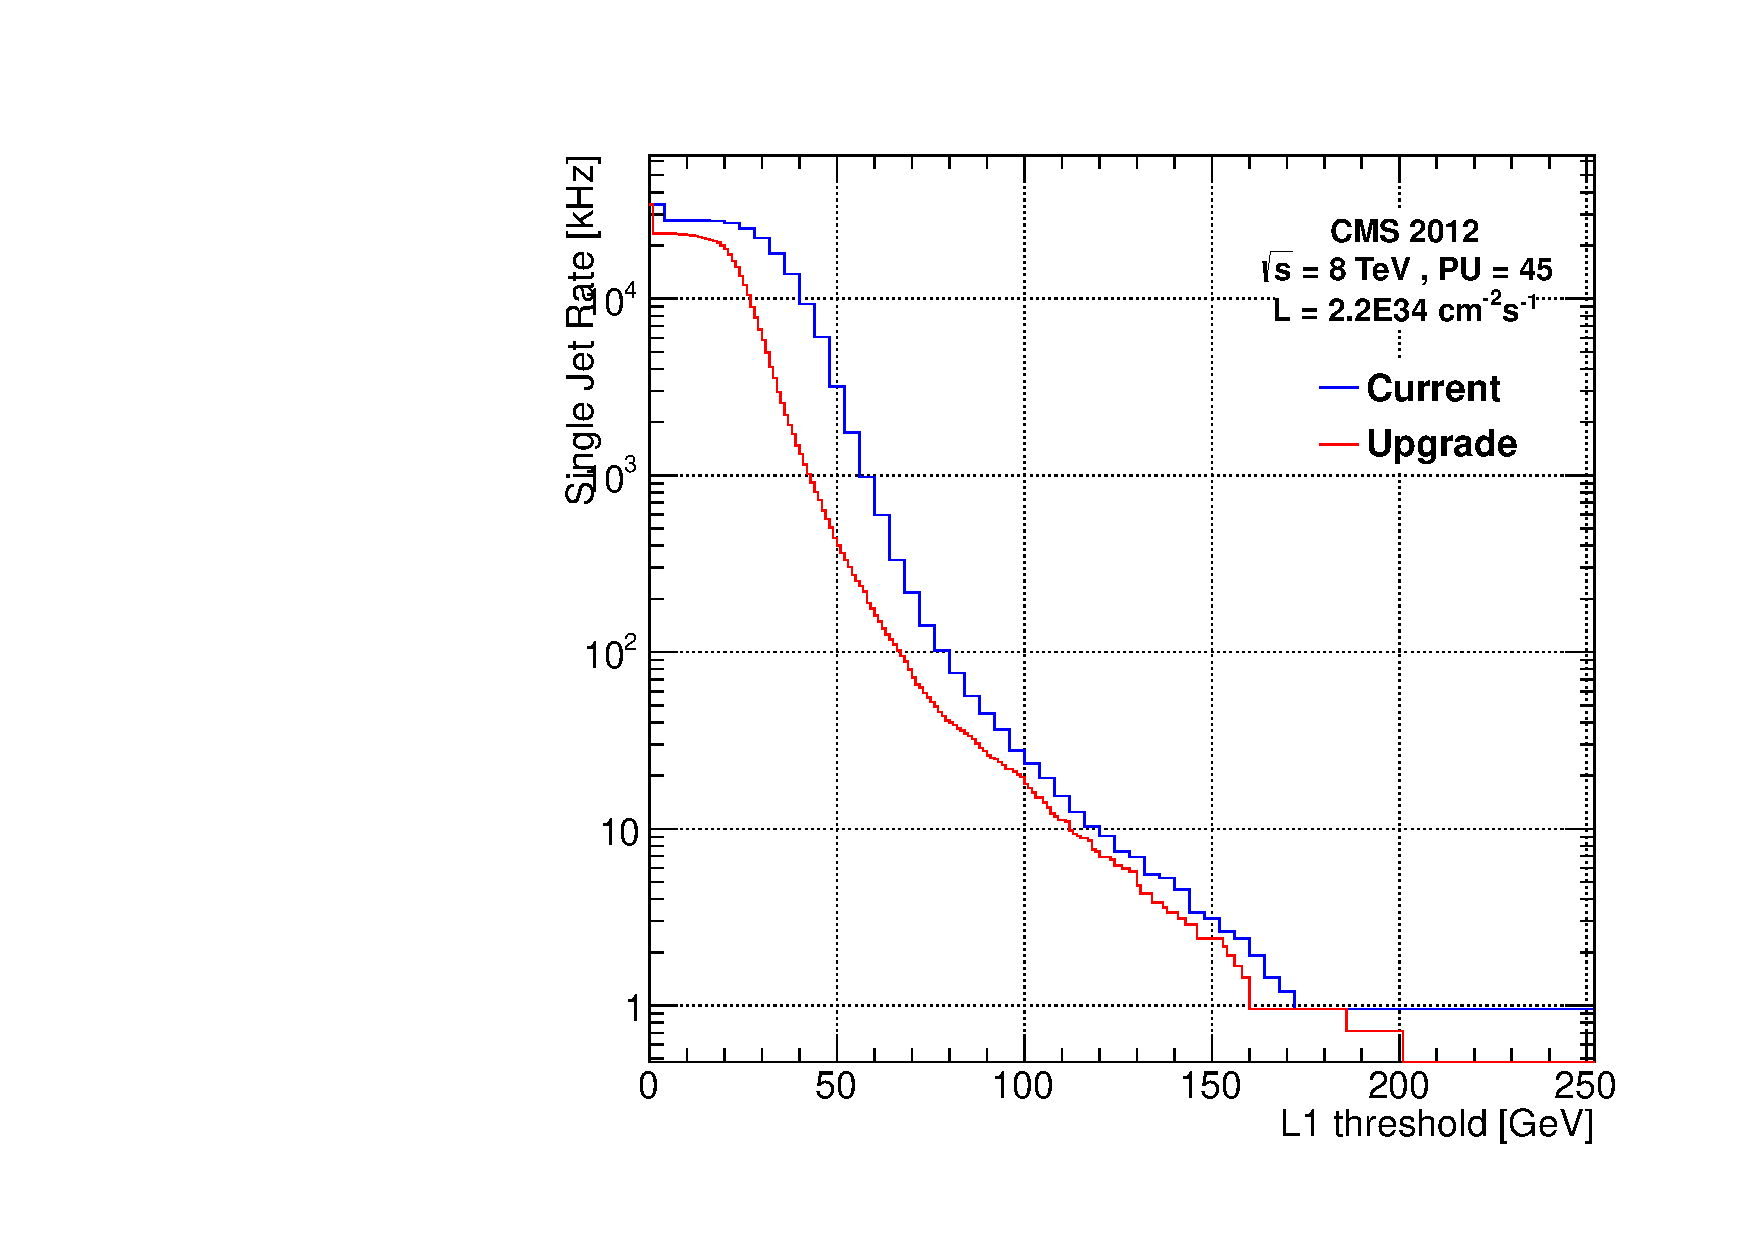
\includegraphics[scale=0.3]{Figures/l1jets/singleJetRates_2e34.pdf}
   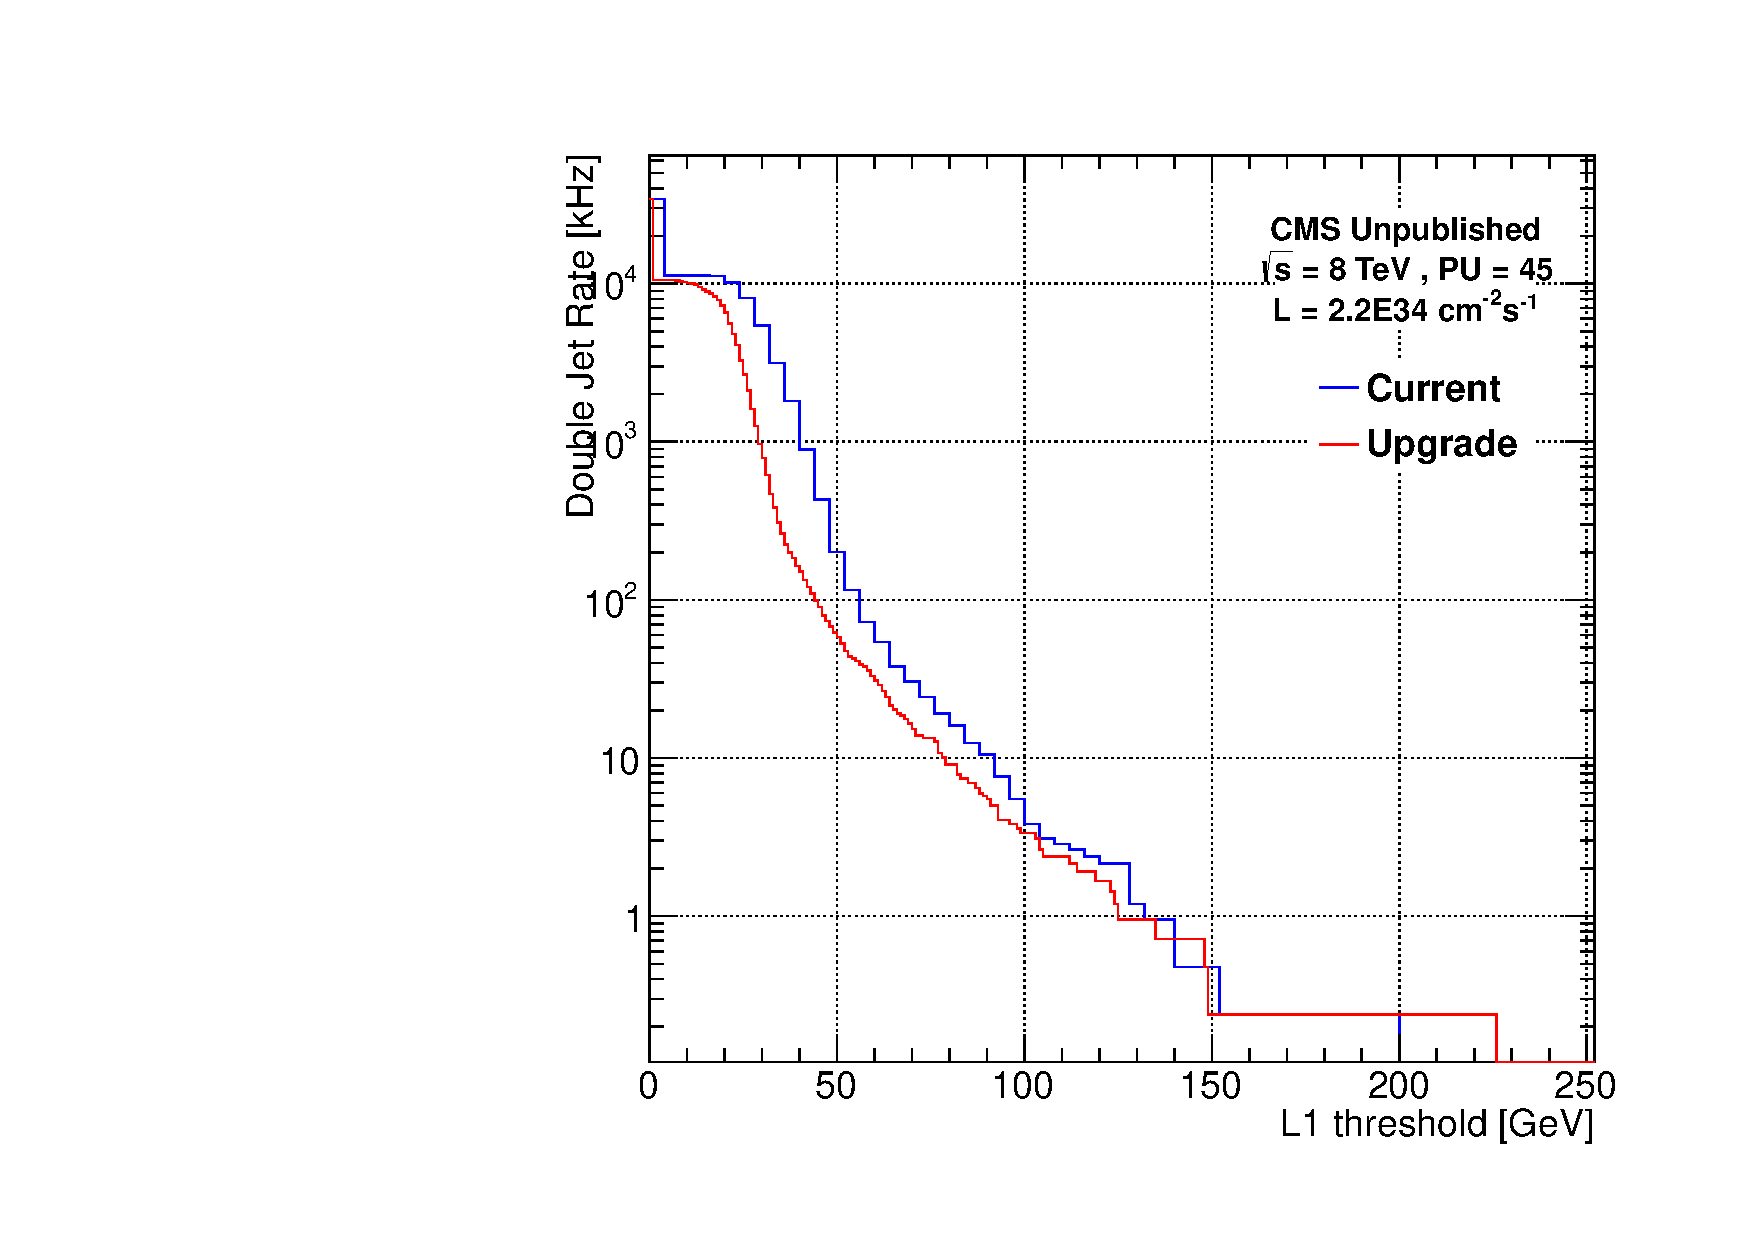
\includegraphics[scale=0.3]{Figures/l1jets/doubJetRates_2e34.pdf}
   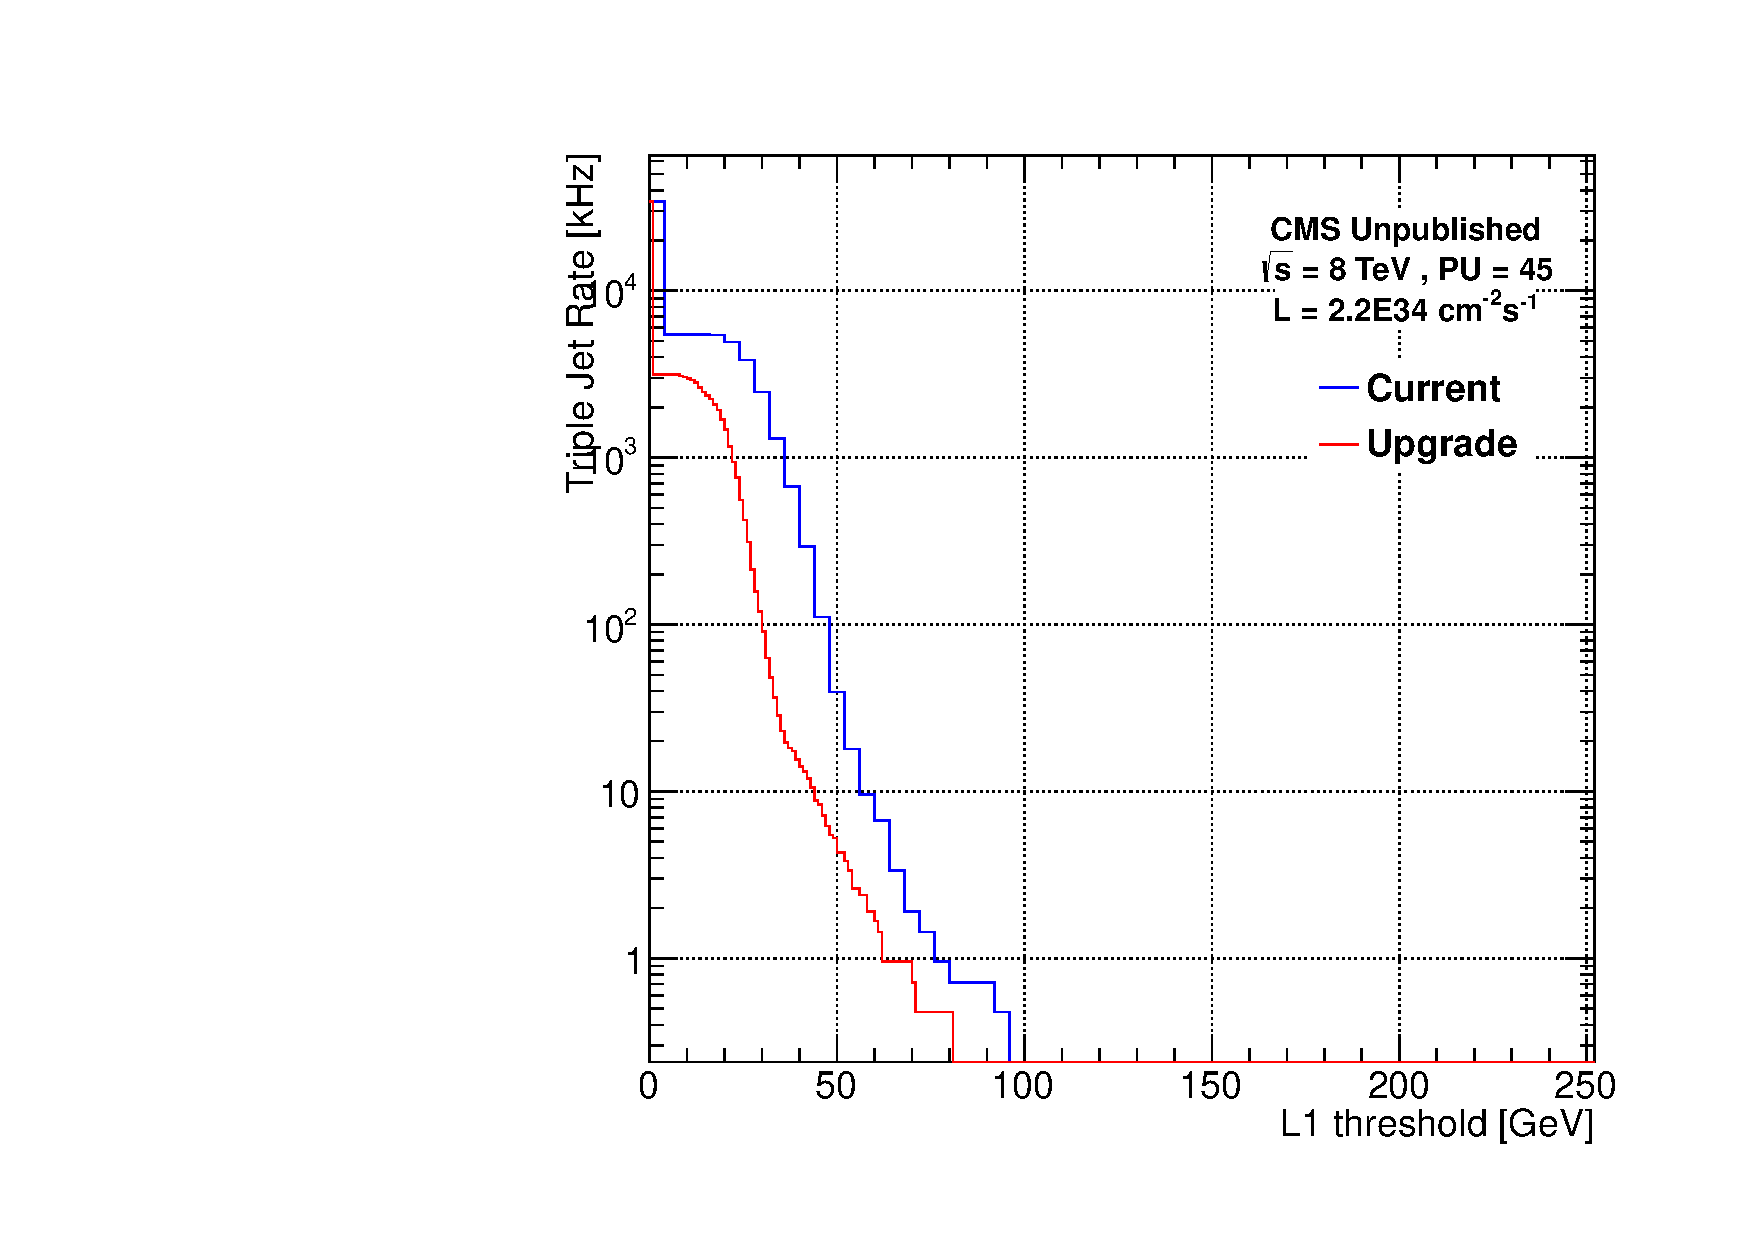
\includegraphics[scale=0.3]{Figures/l1jets/tripJetRates_2e34.pdf}
   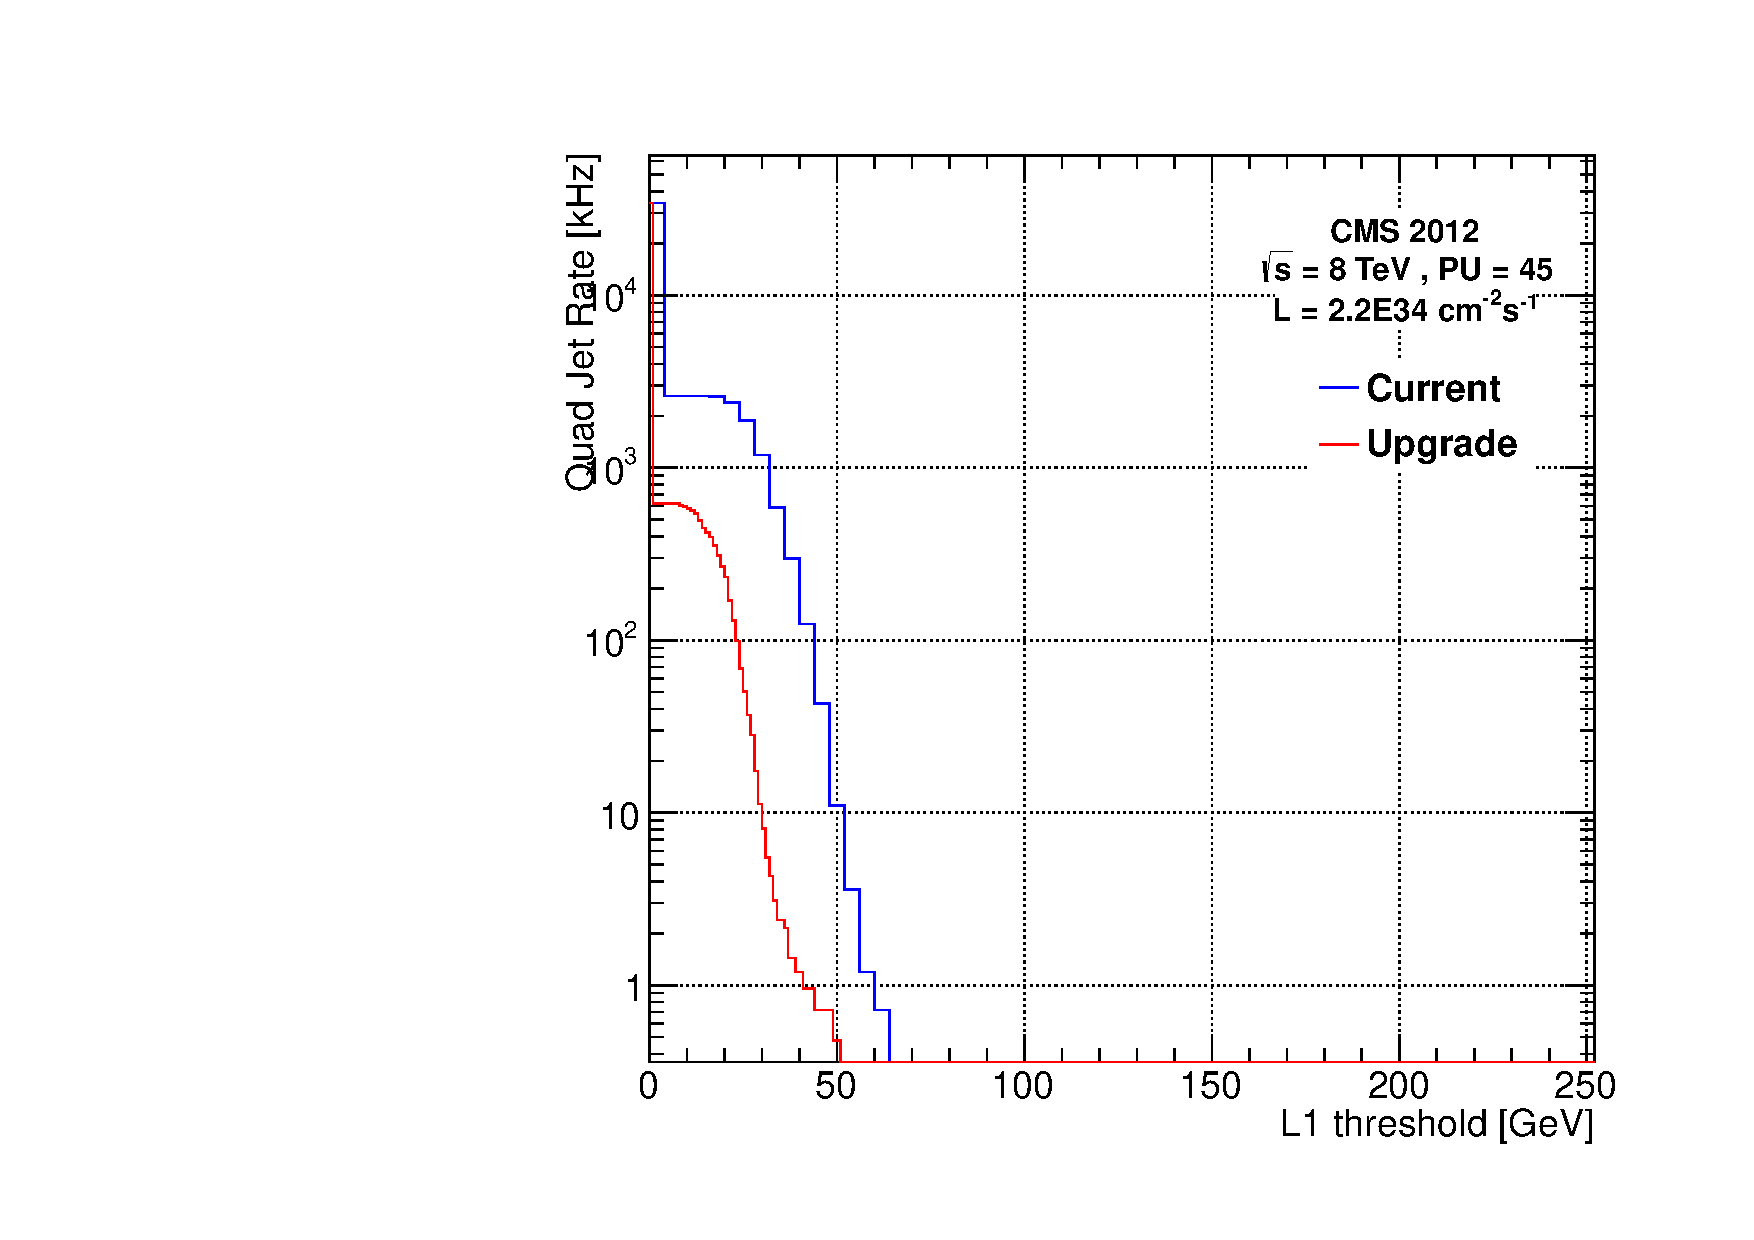
\includegraphics[scale=0.3]{Figures/l1jets/quadJetRates_2e34.pdf}
\caption{Rates of single, double, triple and quad jet triggers. The single jet trigger shows similar performance to the current system, while the multi-jet trigger show a large reduction in rate. }
\label{JetRate_L1}
\end{center}
\end{figure}

\begin{figure}[t!]
%\vspace{-1.cm}
\begin{center}
  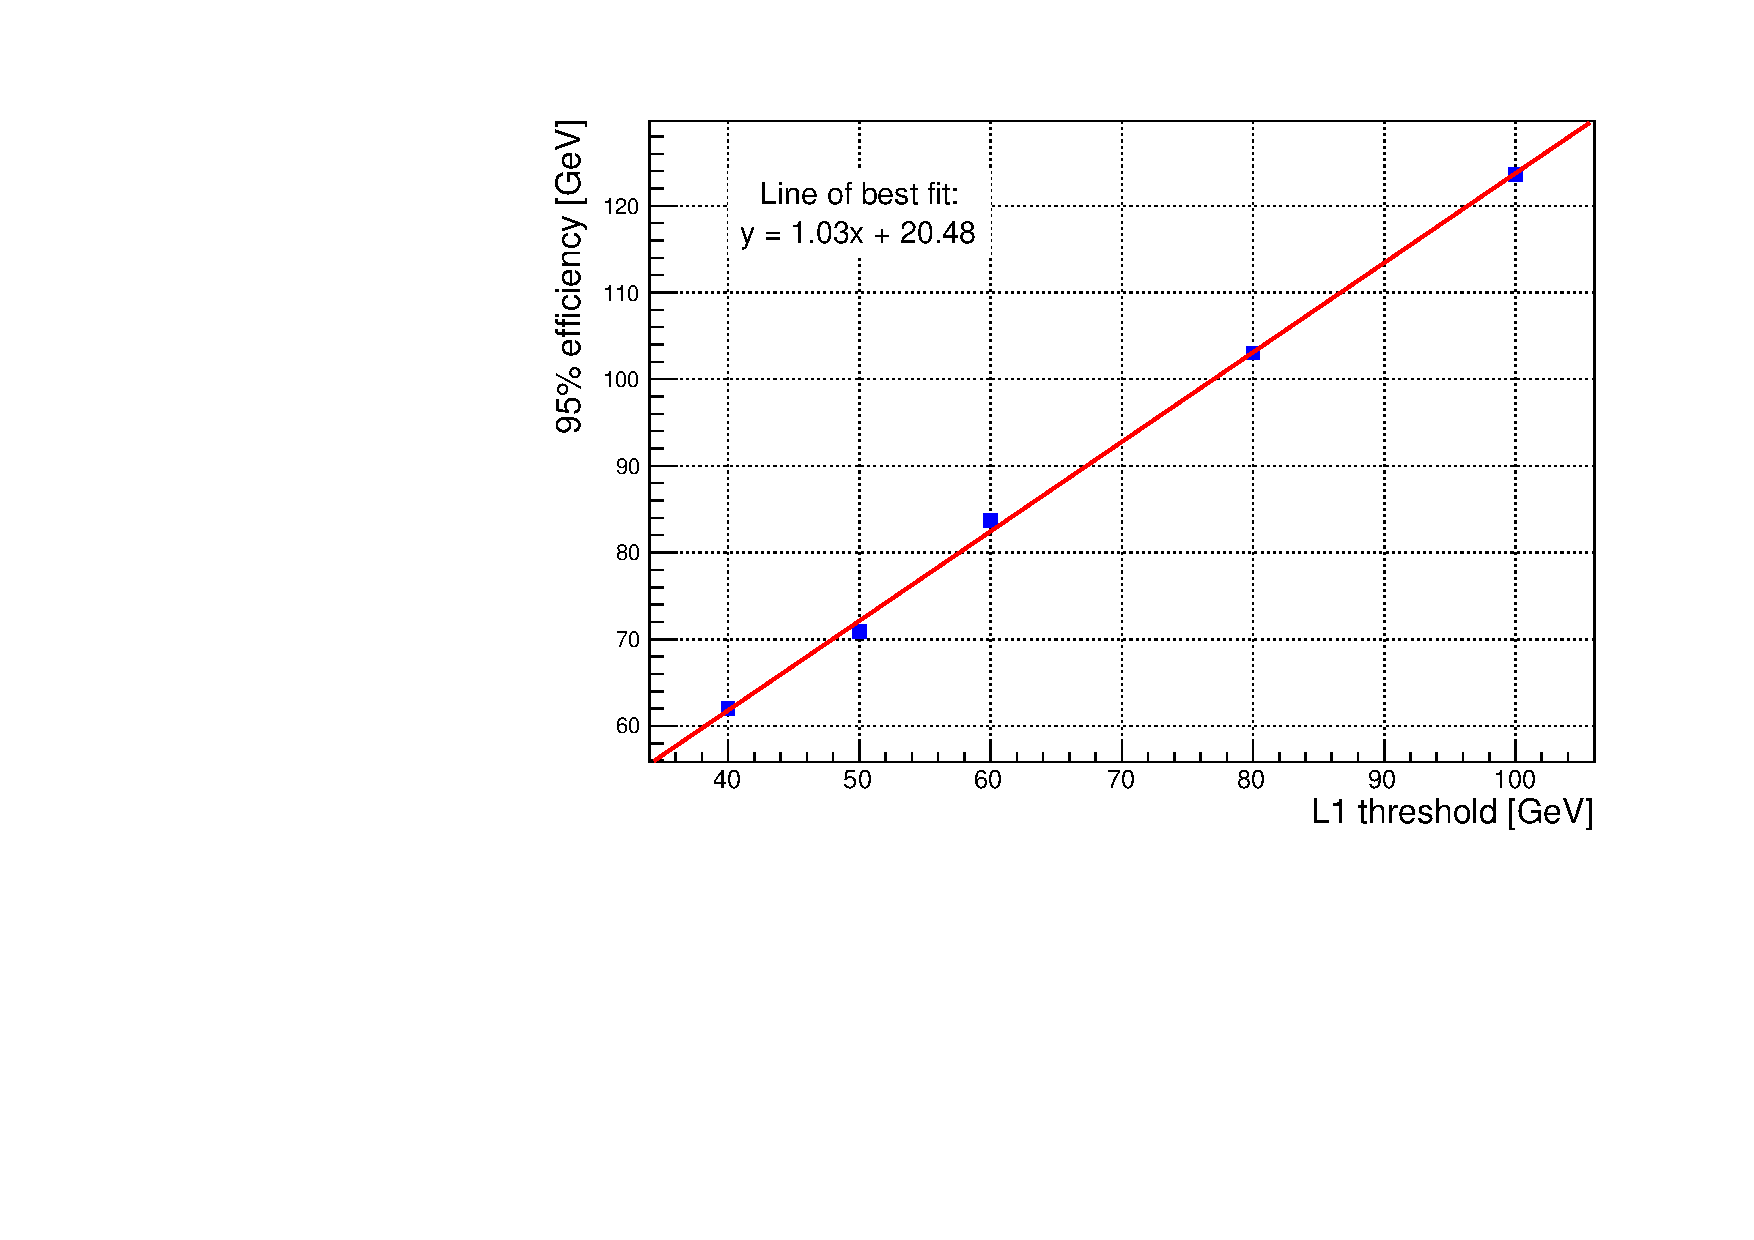
\includegraphics[scale=0.37]{Figures/l1jets/makePlot/jet_95threshold_conv.pdf}
\caption{Conversion between the \ac{L1} jet threshold and the 95\% efficiency as measured offline, for the proposed upgrade jet algorithm, using the turn on curves shown in Figure~\ref{JetTO_highPU}. }
\label{JetRate_conv}
\end{center}
\end{figure}

\begin{figure}[t!]
%\vspace{-1.cm}
\begin{center}
  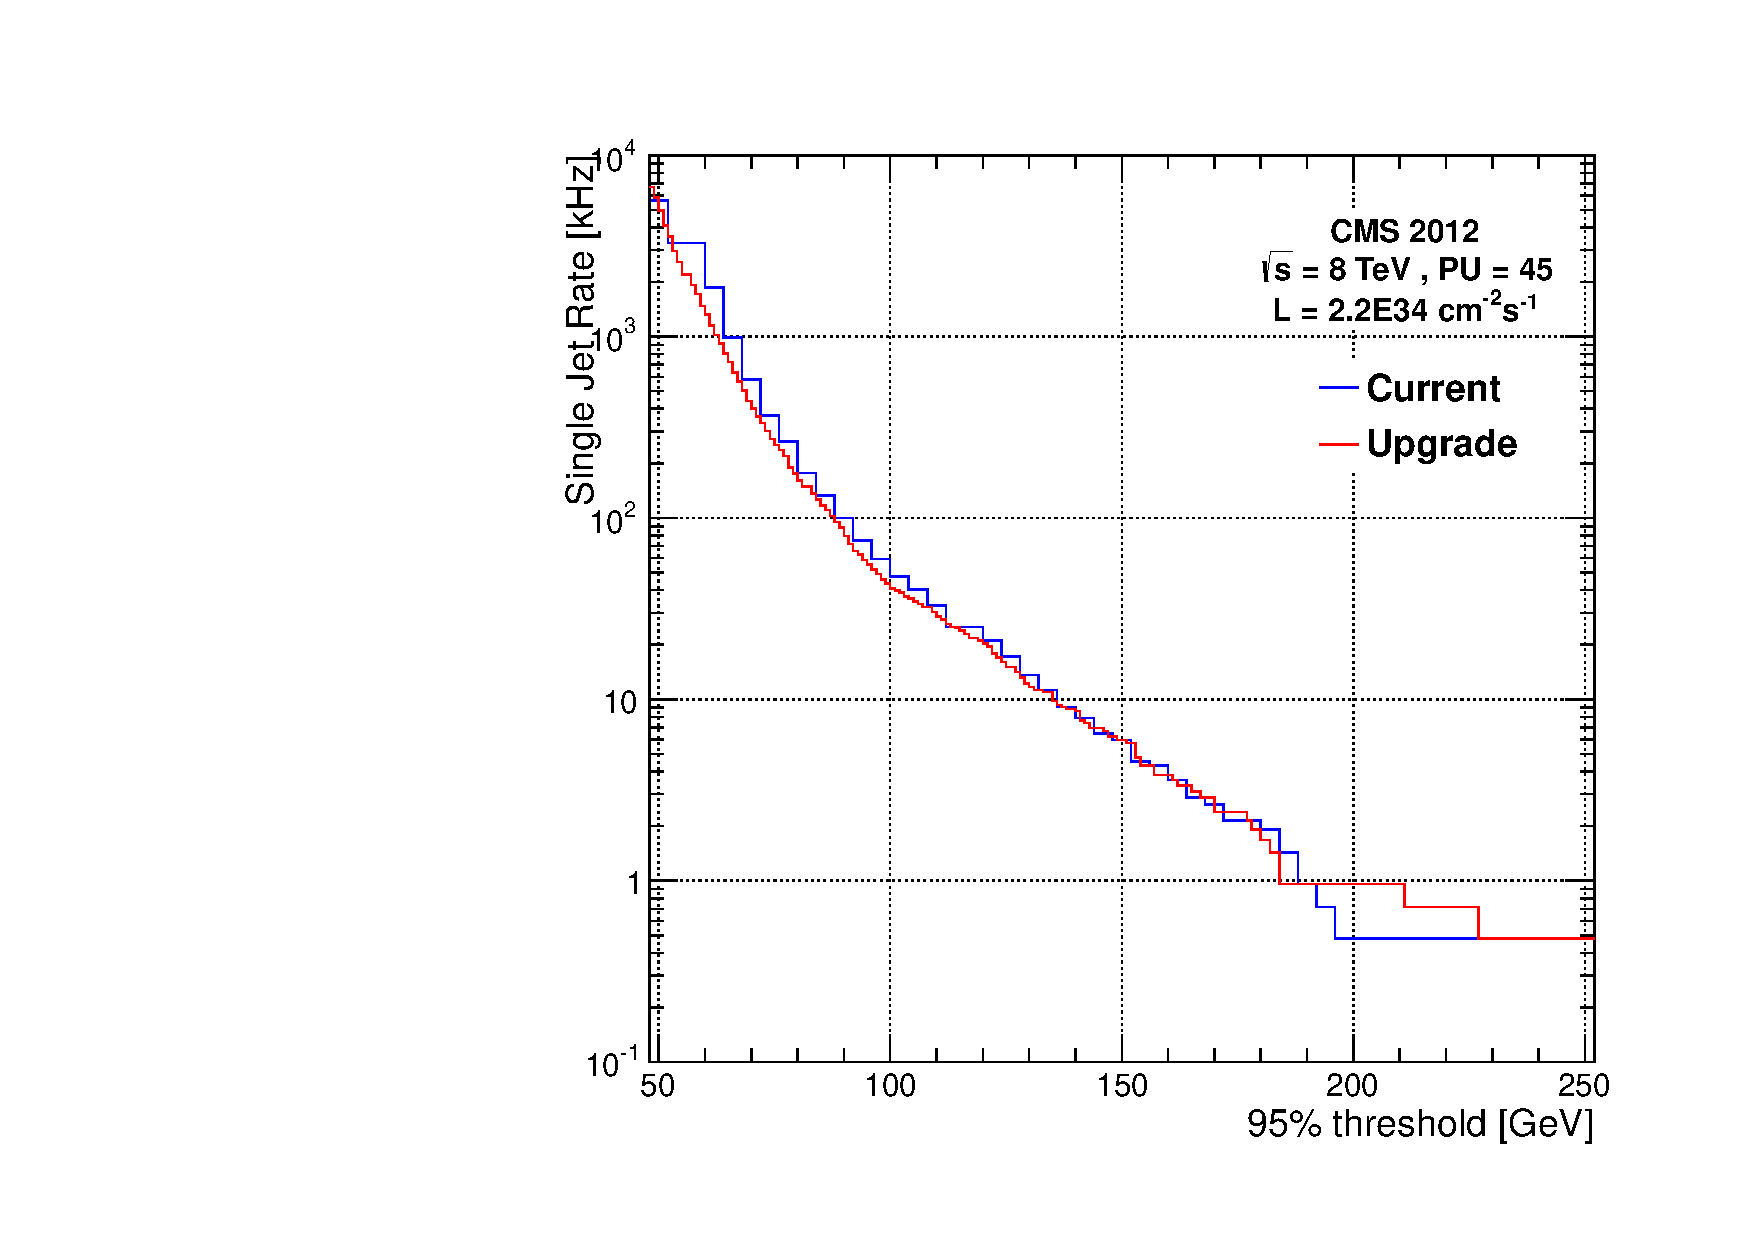
\includegraphics[scale=0.3]{Figures/l1jets/singleJetRates_95thresh_2e34.pdf}
  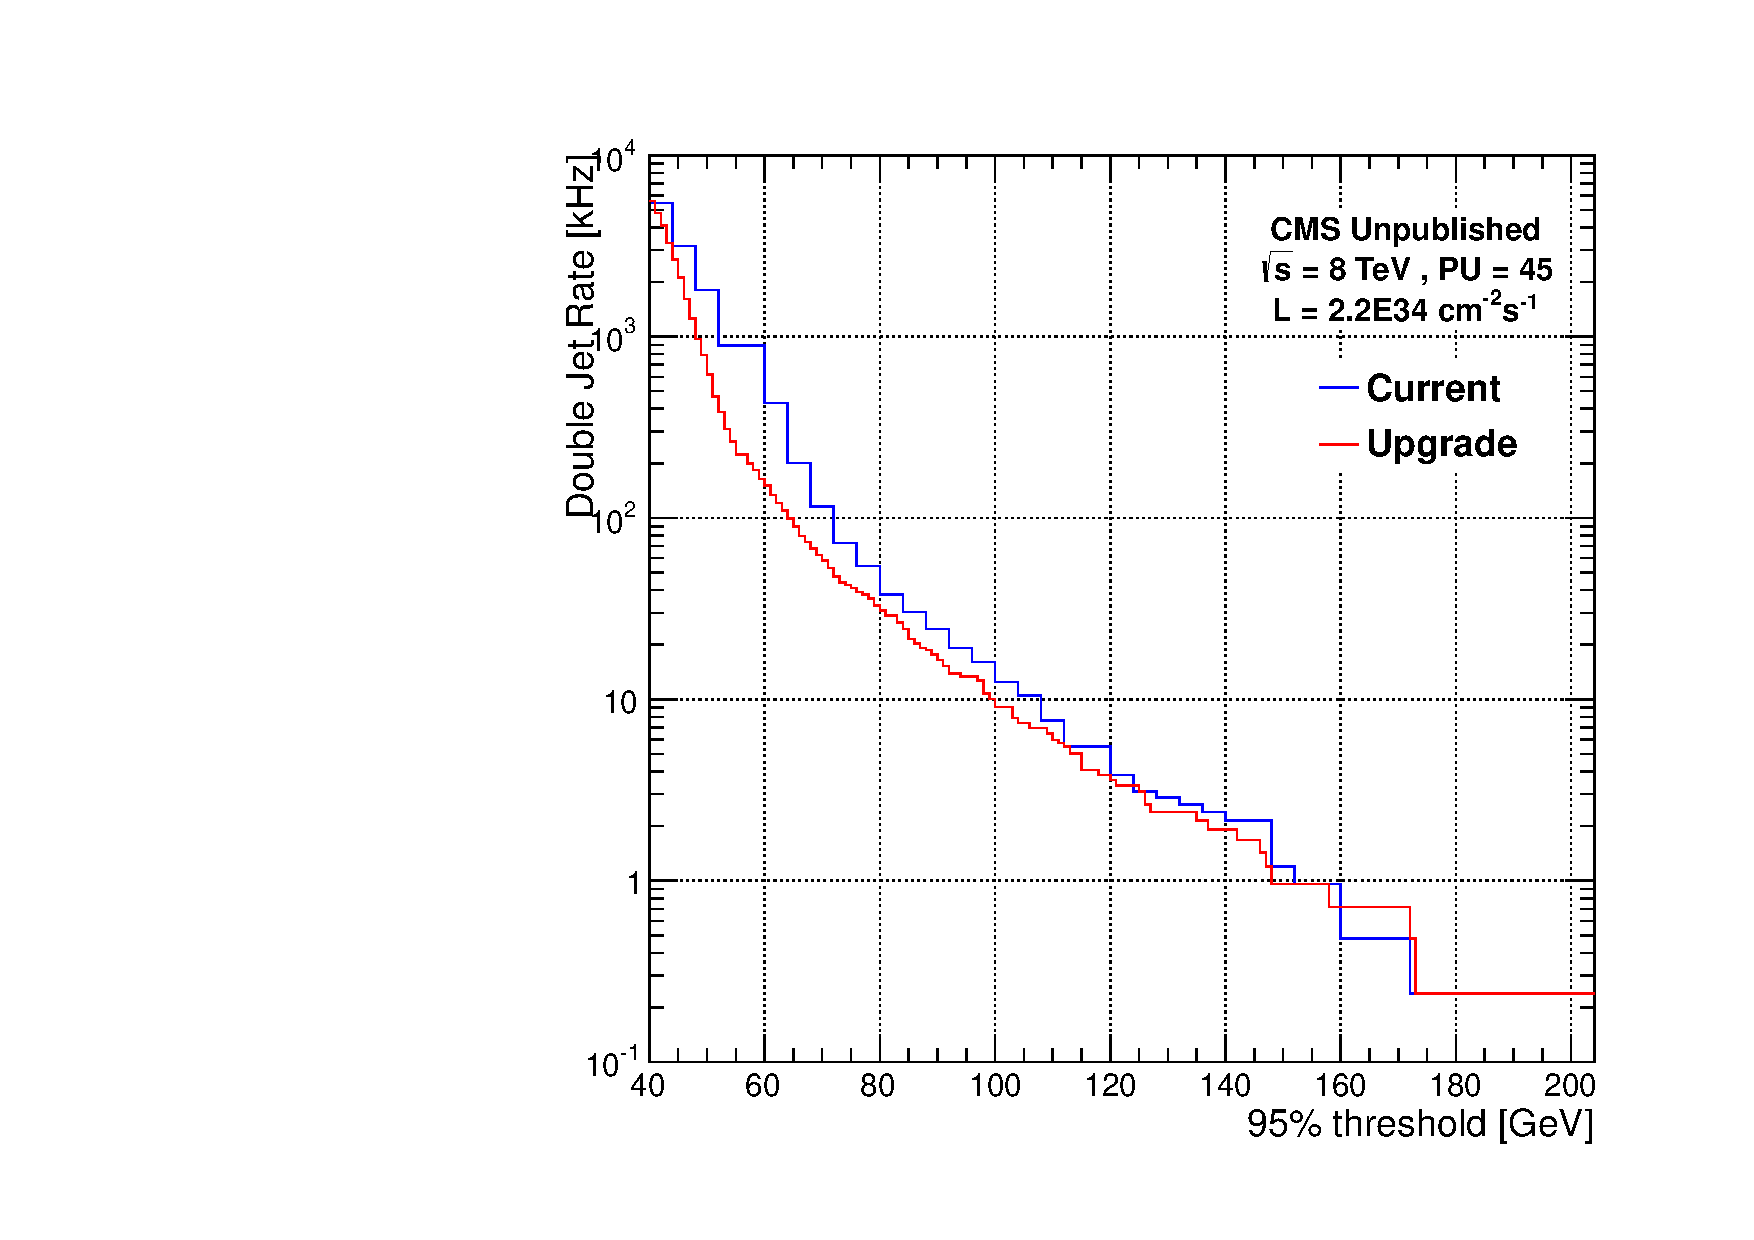
\includegraphics[scale=0.3]{Figures/l1jets/doubleJetRates_95thresh_2e34.pdf}
  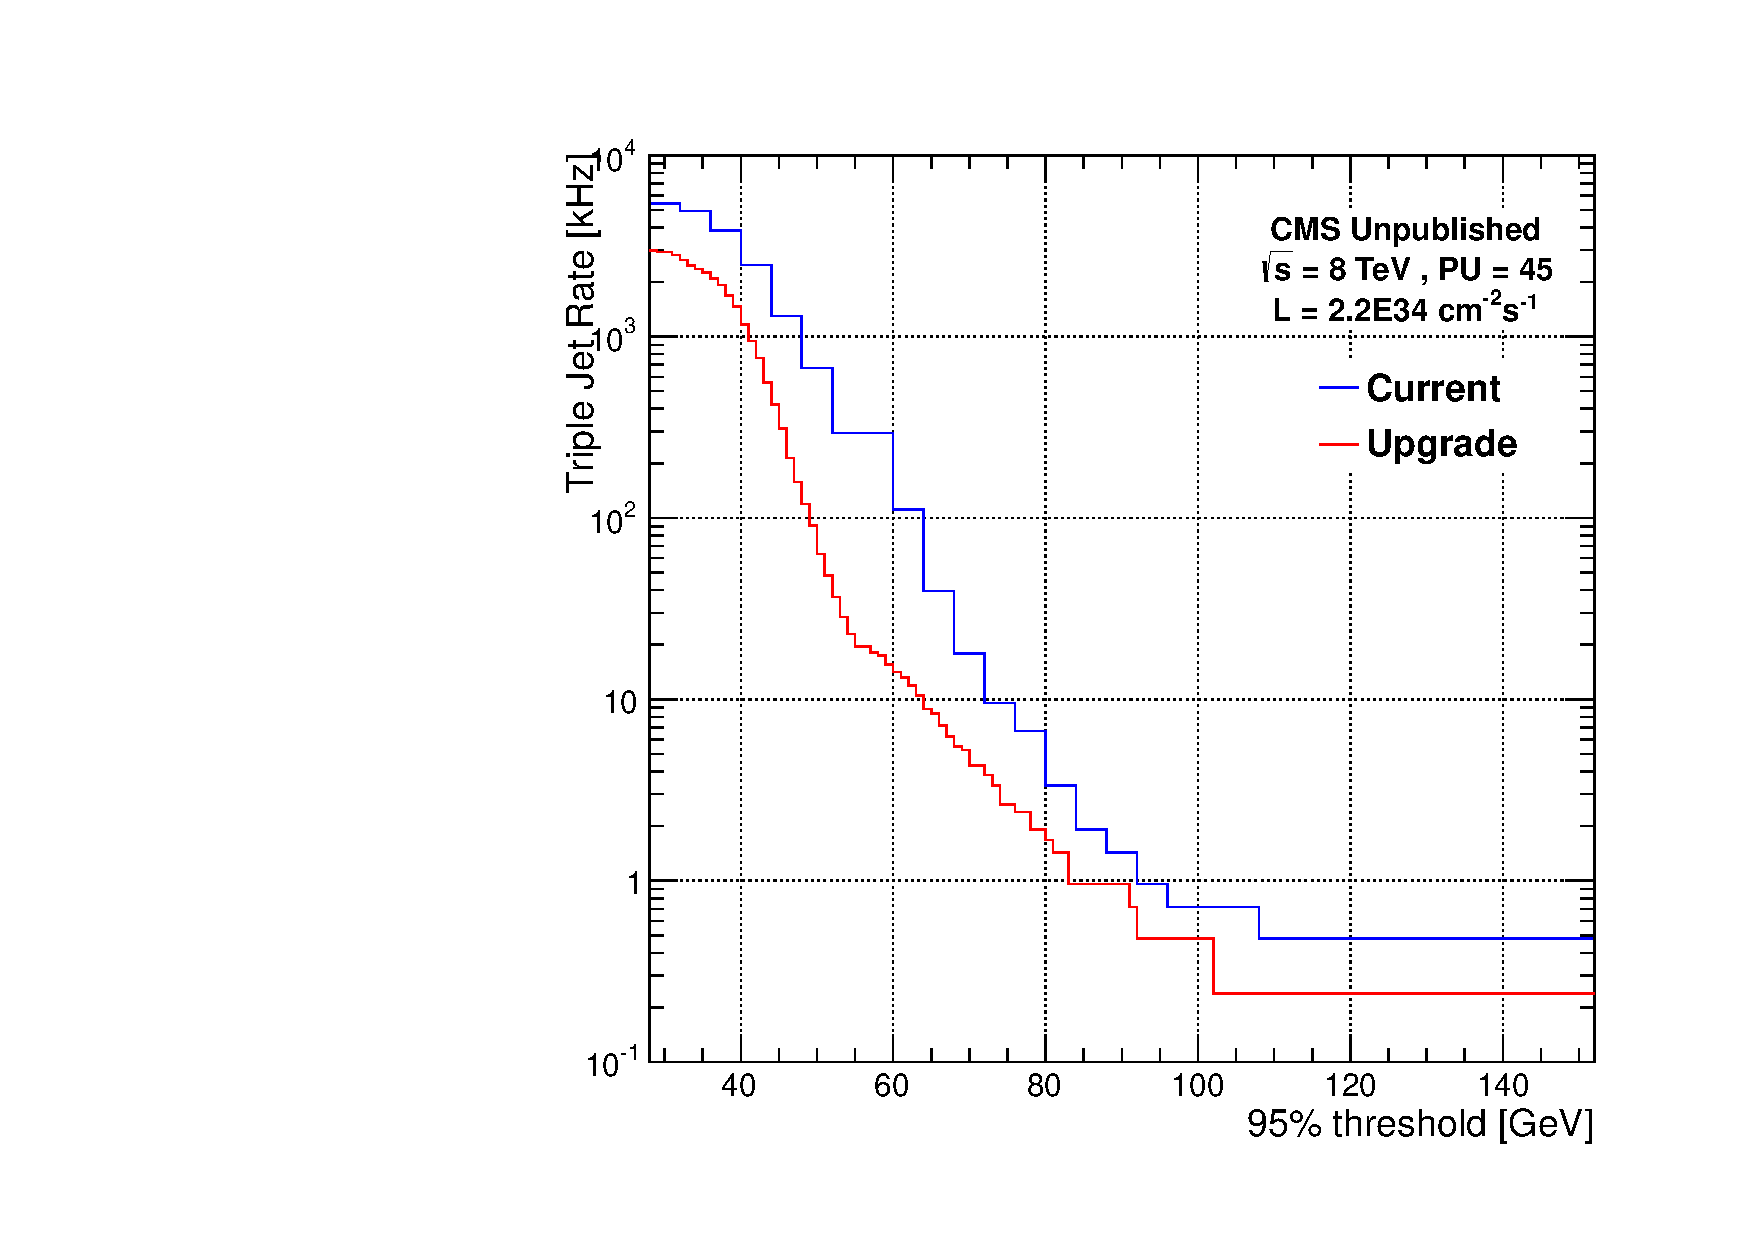
\includegraphics[scale=0.3]{Figures/l1jets/tripleJetRates_95thresh_2e34.pdf}
  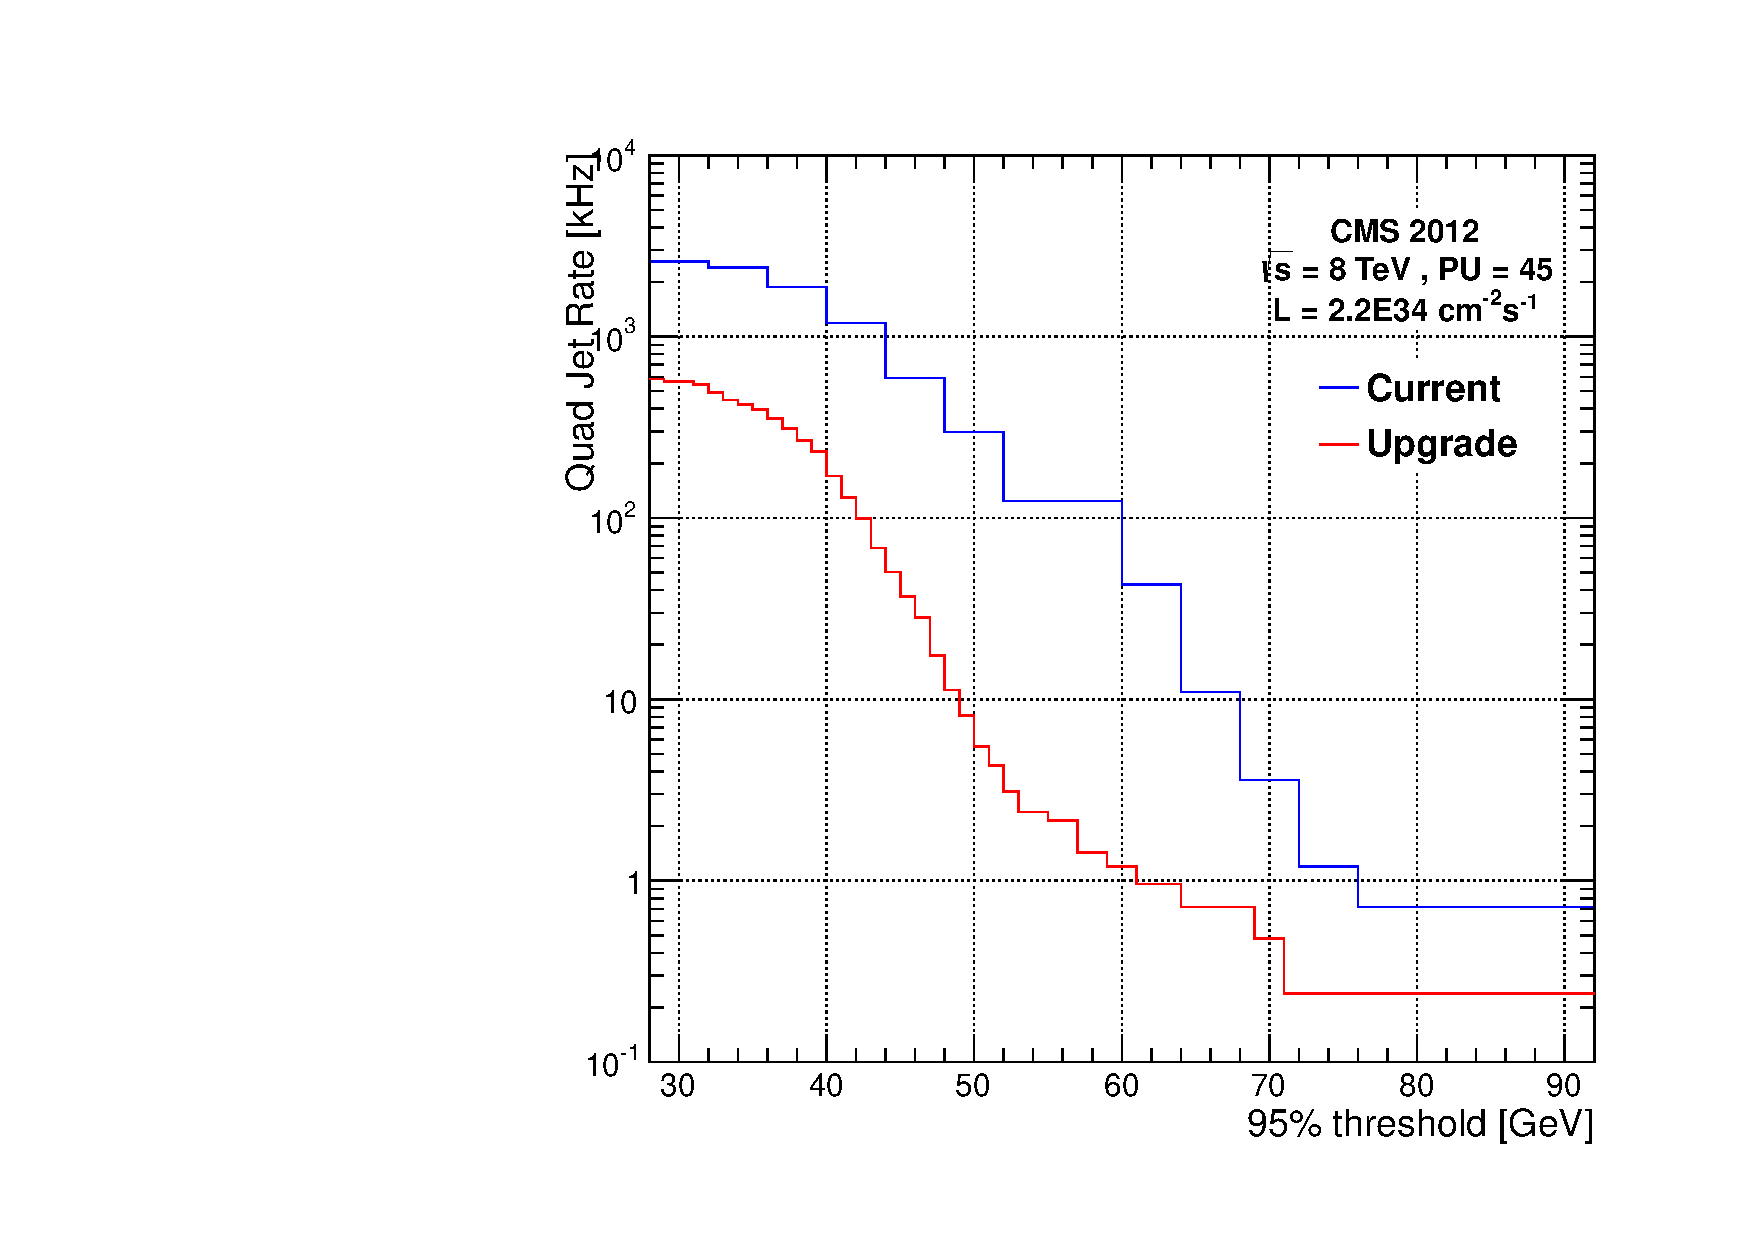
\includegraphics[scale=0.3]{Figures/l1jets/quadJetRates_95thresh_2e34.pdf}
\caption{Rates of single, double, triple and quad jet triggers. The single jet trigger shows similar performance to the current system, while the multi-jet trigger show a large reduction in rate. The single and quad jet rate plots can be found in~\cite{Tapper:1556311}.}
\label{JetRate_95}
\end{center}
\end{figure}


\subsection{Other jet variables}
Other offline variables, constructed from jets, have been widely used in the data analyses at \ac{CMS} at 7 and 8~\TeV, both at trigger level and offline.
They therefore will also benefit from the upgraded calorimeter trigger, and shown here are the improvements in rates for \HT, the transverse hadronic energy which is defined as the scalar sum of jet transverse momenta in each event:
%
\begin{eqnarray}
\HT &=& \sum{|\pt^{\text{ jet}}|} %\\ 
%\MHT &=&  \sum{\ptv^{\text{ jet}}},
\end{eqnarray}  
where the sum is over all jets in each event.
\HT is commonly used in analyses which search for \ac{SUSY}, for example in Ref.~\cite{alphaT}.
It gives a good indication of the amount of hadronic energy in an event and so the energy transfer in the original inelastic pp collision, which should be high for new physics processes to occur.
It is particularly sensitive to the number of primary vertices in each bunch crossing, as soft \ac{PU} jets are included in the sum.
The addition of \ac{PU} subtraction on an event-by-event basis in the proposed upgrade jet algorithm therefore has the potential to lead to significant improvements in the rate.
The trigger turn on curves for various \HT thresholds using the upgrade jet algorithm are shown in Figure~\ref{HTRate_conv} together with the conversion between the \ac{L1} threshold and the 95\% offline efficiency. 
The trigger rate of the \HT in terms of both the \ac{L1} threshold and the 95\% efficiency are shown in Figure~\ref{HTRate}, which shows a rate reduction of nearly an order of magnitude when using the upgrade algorithm compared to the current algorithm, in terms of the 95\% efficiency. 
This is a much fairer comparison between the two algorithms than the rate in terms of the \ac{L1} threshold, as the current \HT \deleted{and \MHT} values at \ac{L1} are not corrected to the jet energy scale.


\begin{figure}[t!]
%\vspace{-1.cm}
\begin{center}
  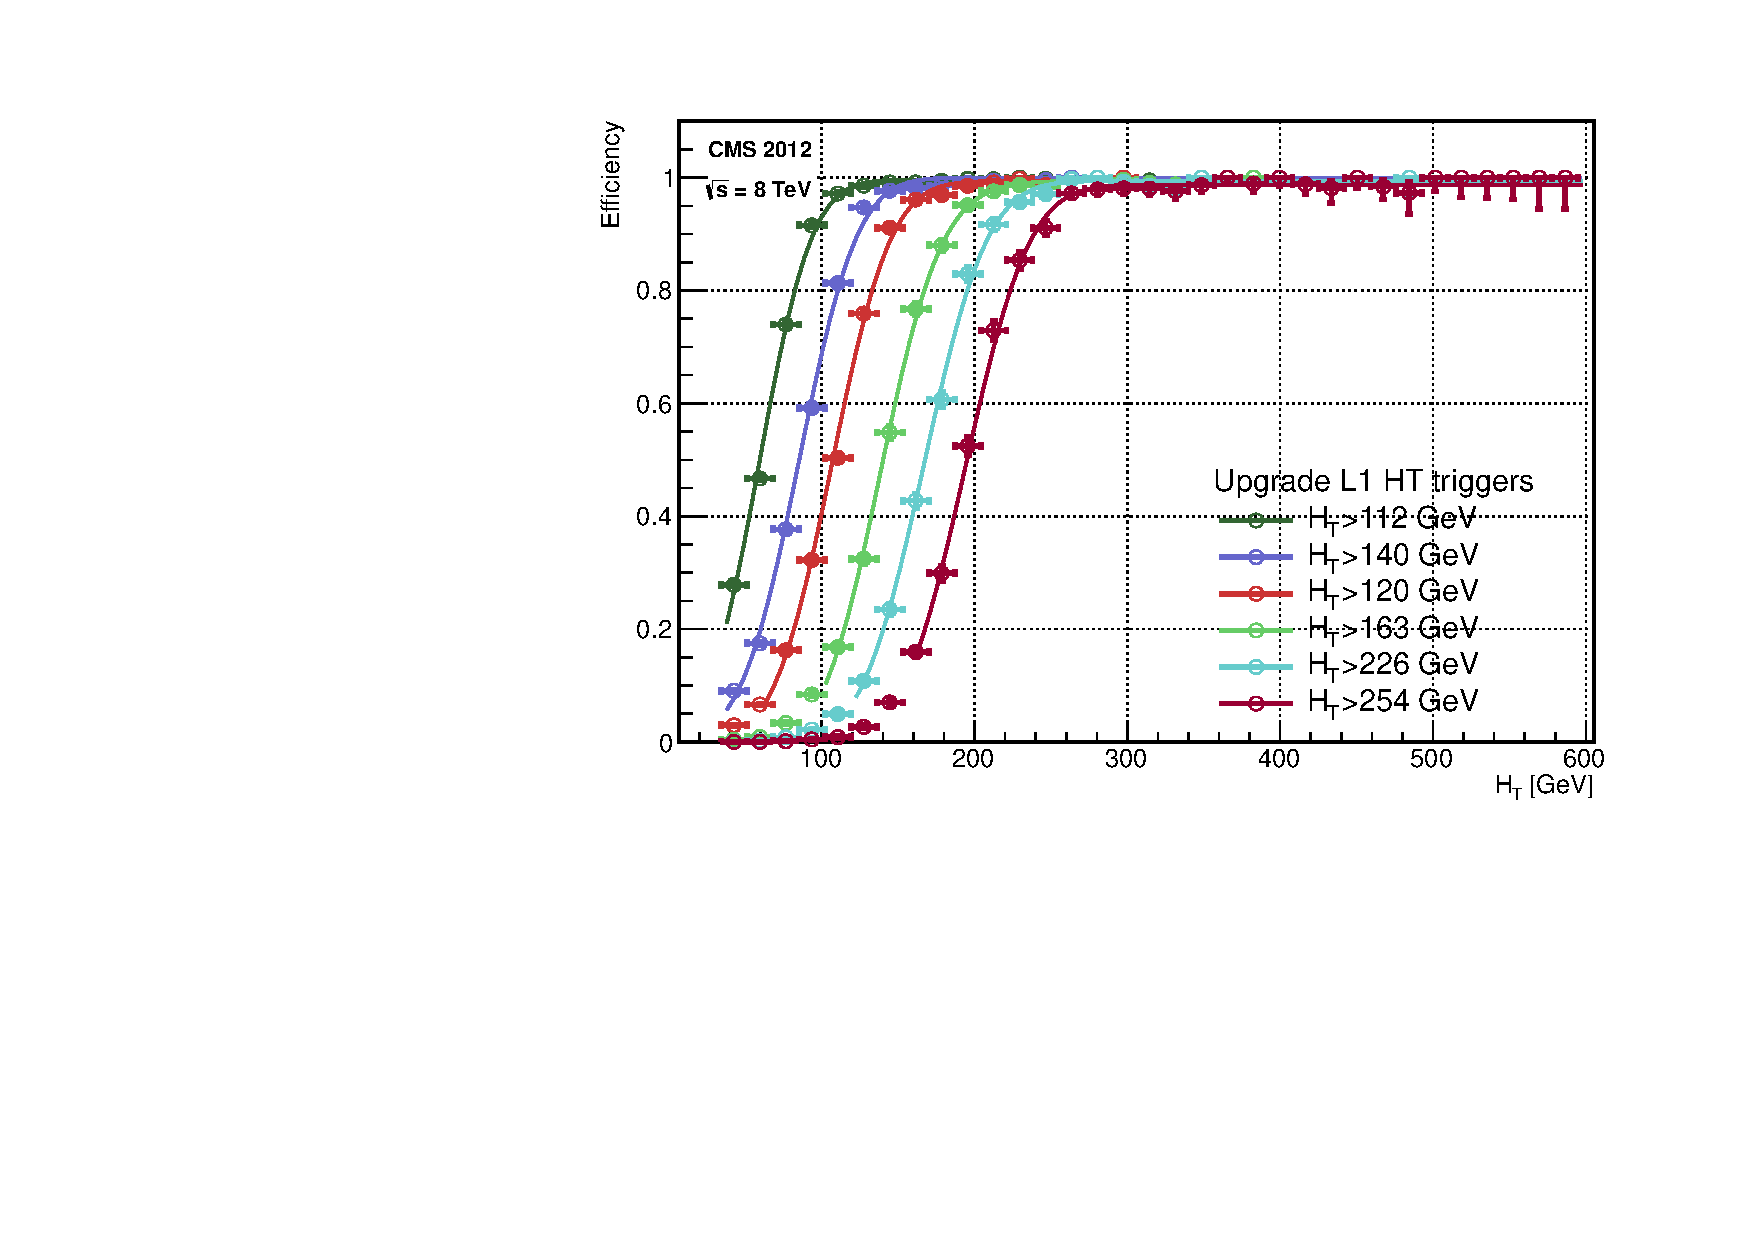
\includegraphics[scale=0.37]{Figures/l1jets/UpgradeL1HTTriggersfixed.pdf}
  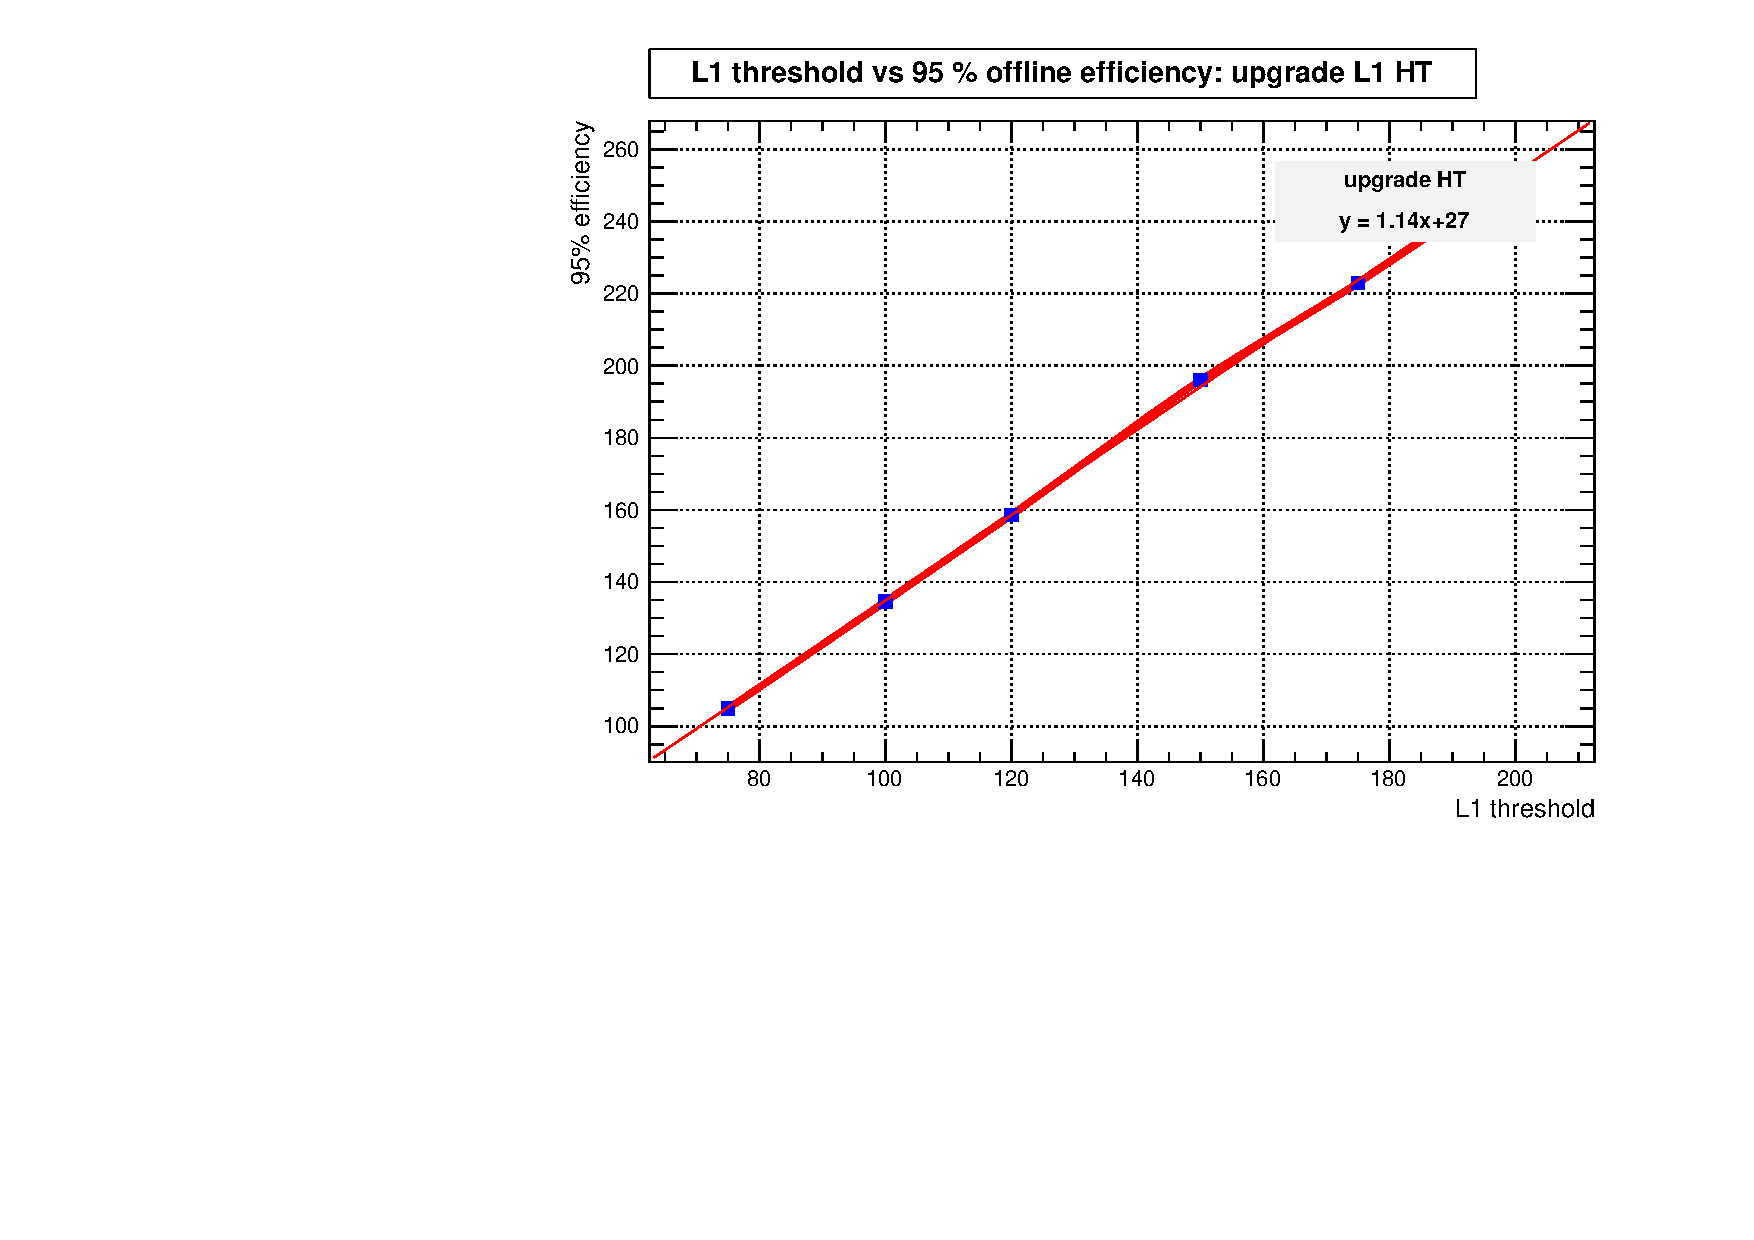
\includegraphics[scale=0.37]{Figures/l1jets/upgradeHTconv.pdf}
\caption{The trigger turn on curves for the \HT variable, left, and the conversion between the \ac{L1} \HT threshold and the 95\% efficiency as measured offline, using \HT constructed with the proposed upgrade algorithm. }
\label{HTRate_conv}
\end{center}
\end{figure}

\begin{figure}[t!]
%\vspace{-1.cm}
\begin{center}
  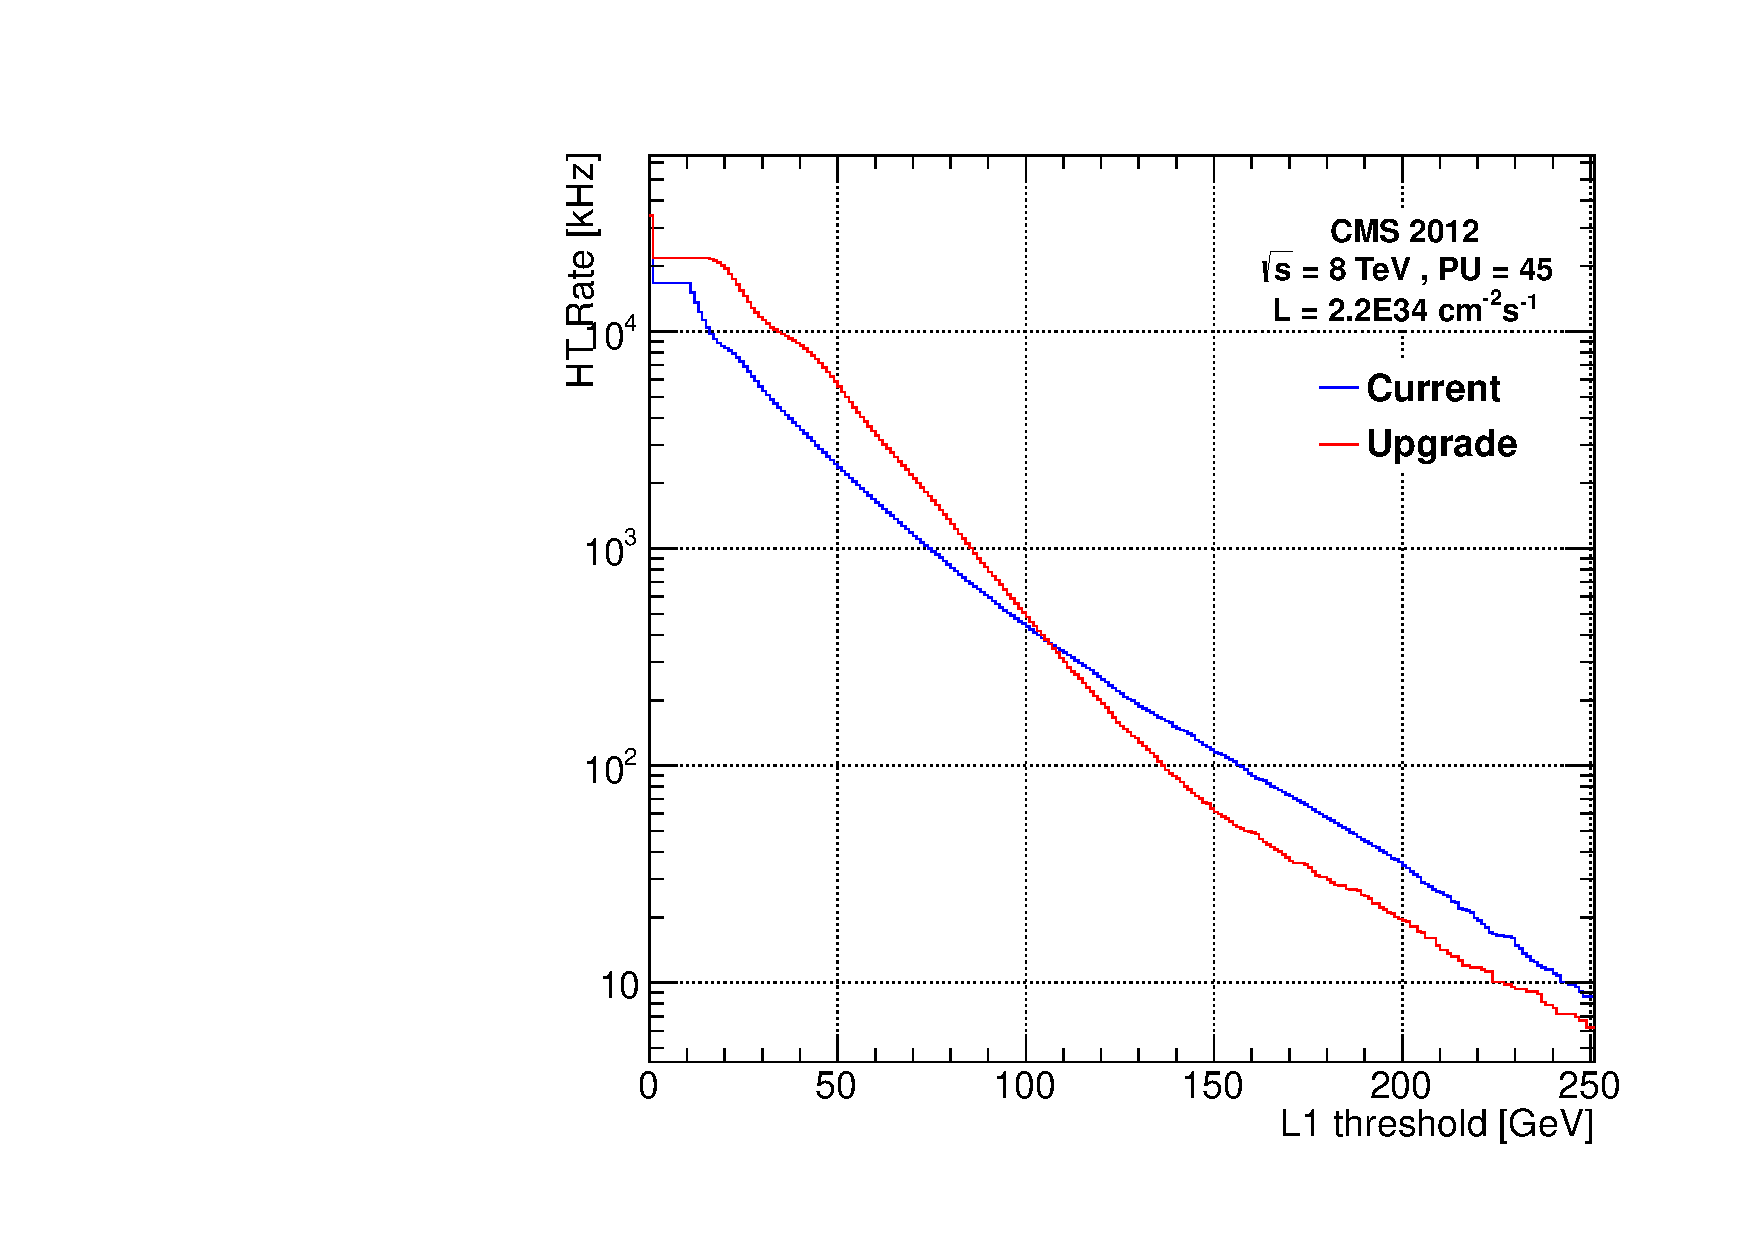
\includegraphics[scale=0.3]{Figures/l1jets/HTRates_2e34.pdf}
    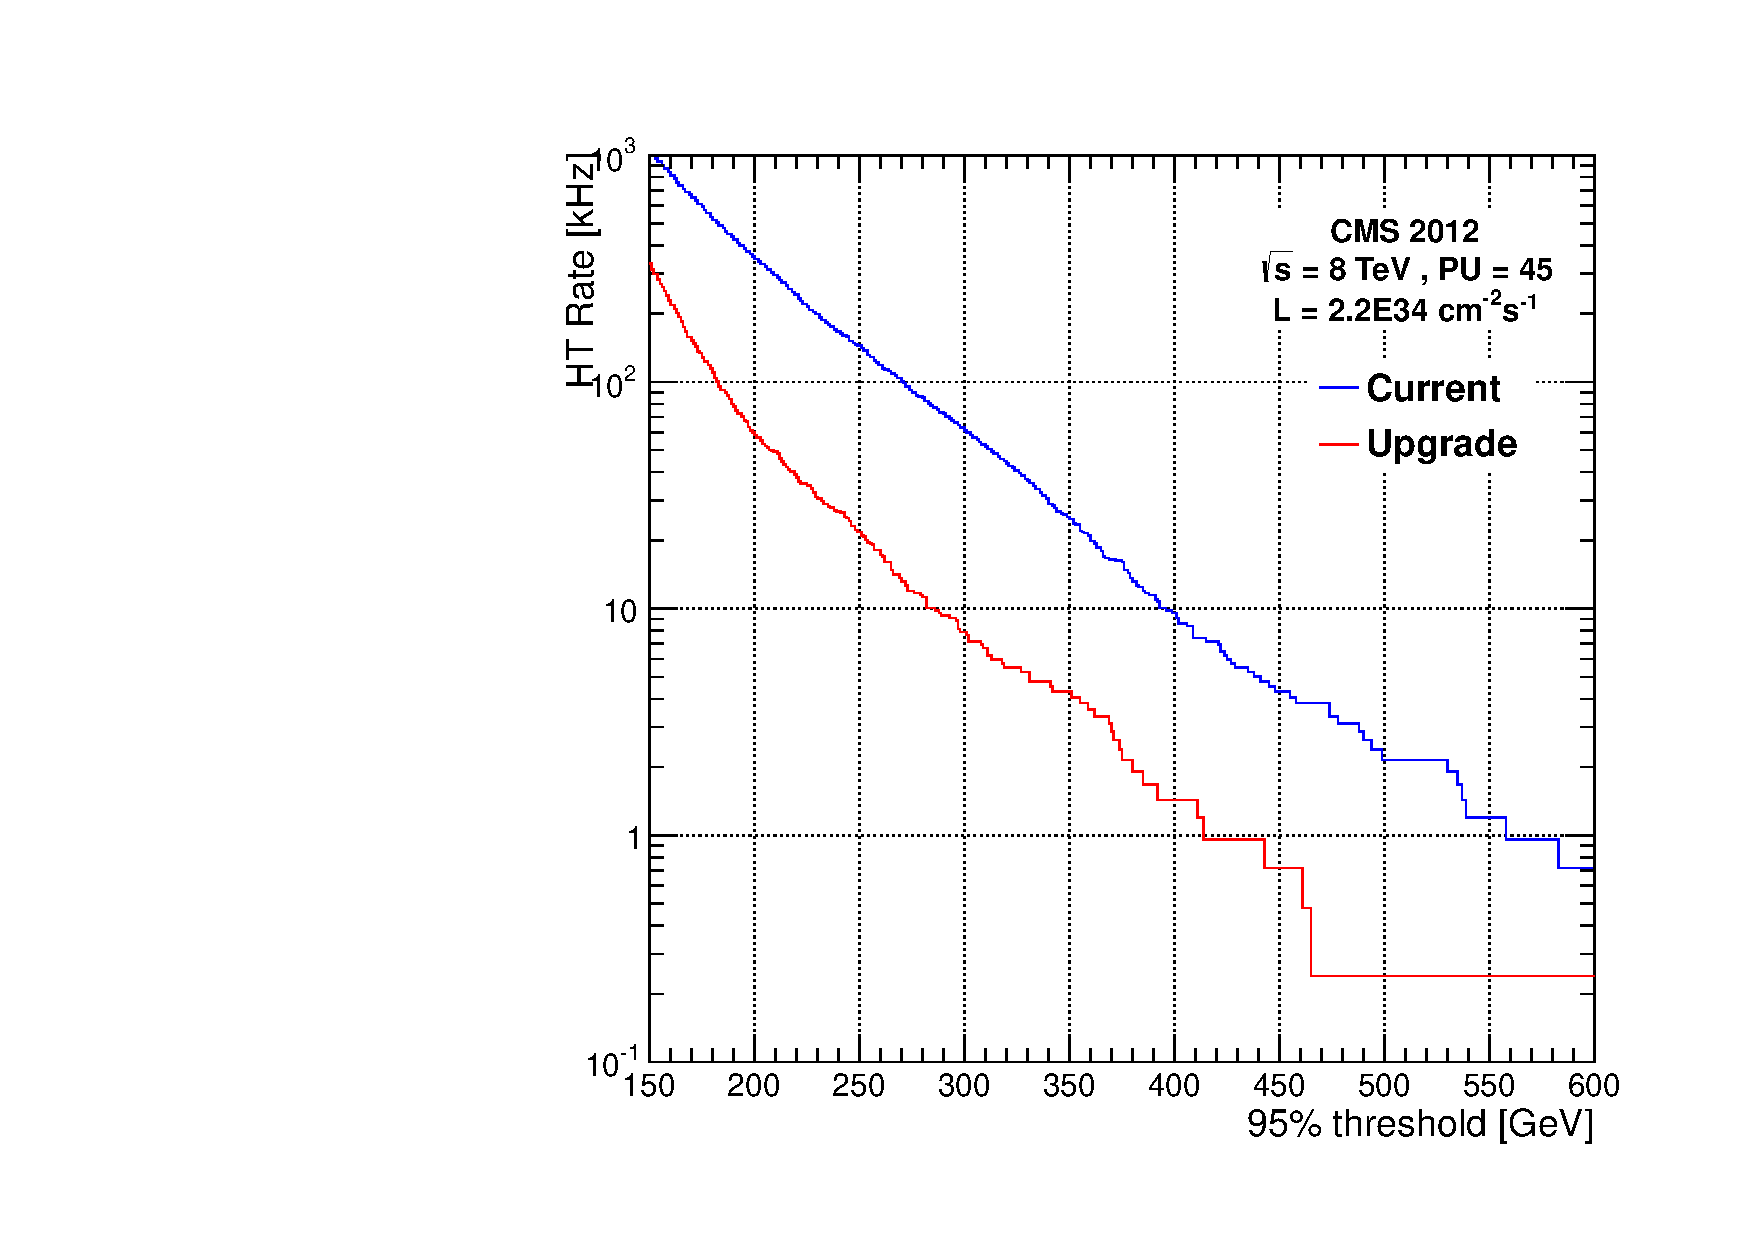
\includegraphics[scale=0.3]{Figures/l1jets/HTRates_95thresh_2e34.pdf}
\caption{Rates of \HT triggers, vs \ac{L1} threshold (left) and 95\% offline threshold (right), where the conversion between \ac{L1} threshold and 95\% efficiency is taken from Figure~\ref{HTRate_conv}. There is a significant reduction in rates with the proposed upgrade algorithm.}
\label{HTRate}
\end{center}
\end{figure}

% The expected enhancement in \MHT is less significant, because it is defined as a vector sum so therefore already has a rudimentary \ac{PU} subtraction applied. 
% However, the rates were nevertheless investigated, and are shown in Figure~\ref. 
 

\section{Conclusion}
The proposed upgrade jet algorithm, which is possible to implement with the upgraded \ac{CMS} calorimeter trigger based upon a \ac{TMT} architecture, shows significant improvements over the current \ac{L1} jet algorithm.
By utilising event-by-event \ac{PU} subtraction at \ac{L1} for the first time, the dependency of \ac{PU} of the \ac{L1} jet algorithm is much reduced.
By taking advantage of the full tower level granularity of the calorimeter, the angular resolutions of the algorithm are also much improved.
This will lead to large improvements in topological calculations at the \ac{GT}, where two or more objects are used to calculate some quantity which is used in triggering; for example transverse mass, and determining jets arising from Vector Boson Fusion processes such as Higgs boson production.
While similar trigger rates are seen for the single jet triggers, there are big improvements in the multijet trigger rates. 
\added{
The double jet rate is reduced by a factor of around 2, the triplet jet rate by a factor of about 3, and the quad-jet trigger rate is reduced by a factor of about 4.
}\deleted{and a factor of two reduction in the quad-jet trigger rate.}
The \HT variable sees a factor 10 reduction in rate.
These rate reductions will allow lower energy thresholds in the upgraded \ac{CMS} \ac{L1} calorimeter trigger, as compared to the current \ac{L1} jet algorithm, and help to maintain the energy thresholds and jet rates that were used in 7 and 8~\TeV data taking.


This upgrade jet algorithm was proposed in Ref.~\cite{Tapper:1556311}, and the majority of the work was done during 2012. 
Many improvements to the algorithm are possible, using different \ac{PU} subtraction techniques, different jet shapes, and additional parameters such as jet substructure variables.
Indeed, since this work was completed improvements have been made, and documented elsewhere~\cite{recentL1jetWork}.

\clearpage